%TODO: where should we use this: problems of optical flow methods yield bad segmentations. known problems: large displacements, sharp discontinuities, accuracy for the occlusion detection.
% TODO mention pipeline assumptions
% TODO mention in which language the individual parts are coded.
% TODO check where this might belong to: the color values are stored as CIE lab color images.
% TODO: keep me: Before going into details, let us first revisit the definition of a trajectory. By the term trajectory we refer to a list of tracking points, which is ordered by the frame index in which each point was traced. Therefore, every points knows to which frame it belongs to.
\chapter{Motion Segmentation Pipeline}
In this chapter we explain in detail the relevant stages of our motion segmentation pipeline. For this purpose we heavily rely on the definitions of \textit{Optical Flow} and \textit{Spectral Clustering} introduced in the previous chapter. We start by restating the initial problem statement our pipeline tries to solve. Moreover, for each stage, we describe its required input data and what output it generates. Lastly, we also mention all assumptions and induced limitations for each pipeline stage. \\ \\
The problem statement our pipeline solves is defined as follows: Given a sequence of frames that form a video and their associated depth maps. Then, our goal is to segment the images into regions that mask regions of coherent and independent rigidly moving objects. Therefore, we describe implementation of a motion segmentation pipeline that addresses this problem statement by using optical flows. Moreover, our implementation should be robust according to complex camera movement and noise, should be able to deal with occlusions and missing data, should be able to handle many moving objects, and lastly, it should be able to detect several and fast moving rigid object. \\ \\
The idea of such a segmentation is to identify and extract meaningful rigid motions from a steady background. The motion of an object in a video sequence can usually not be considered as independent in a per frame basis, since typical object motions proceed over a series of frame. From the previous chapter we know that using optical flows enables us to run a consistent tracking of feature points in a video. Hence, the optical flow is an ideal cue for making motion grouping decisions. In our case we use the flows to generate motion point trajectories.
\begin{figure}[H]
\begin{center}
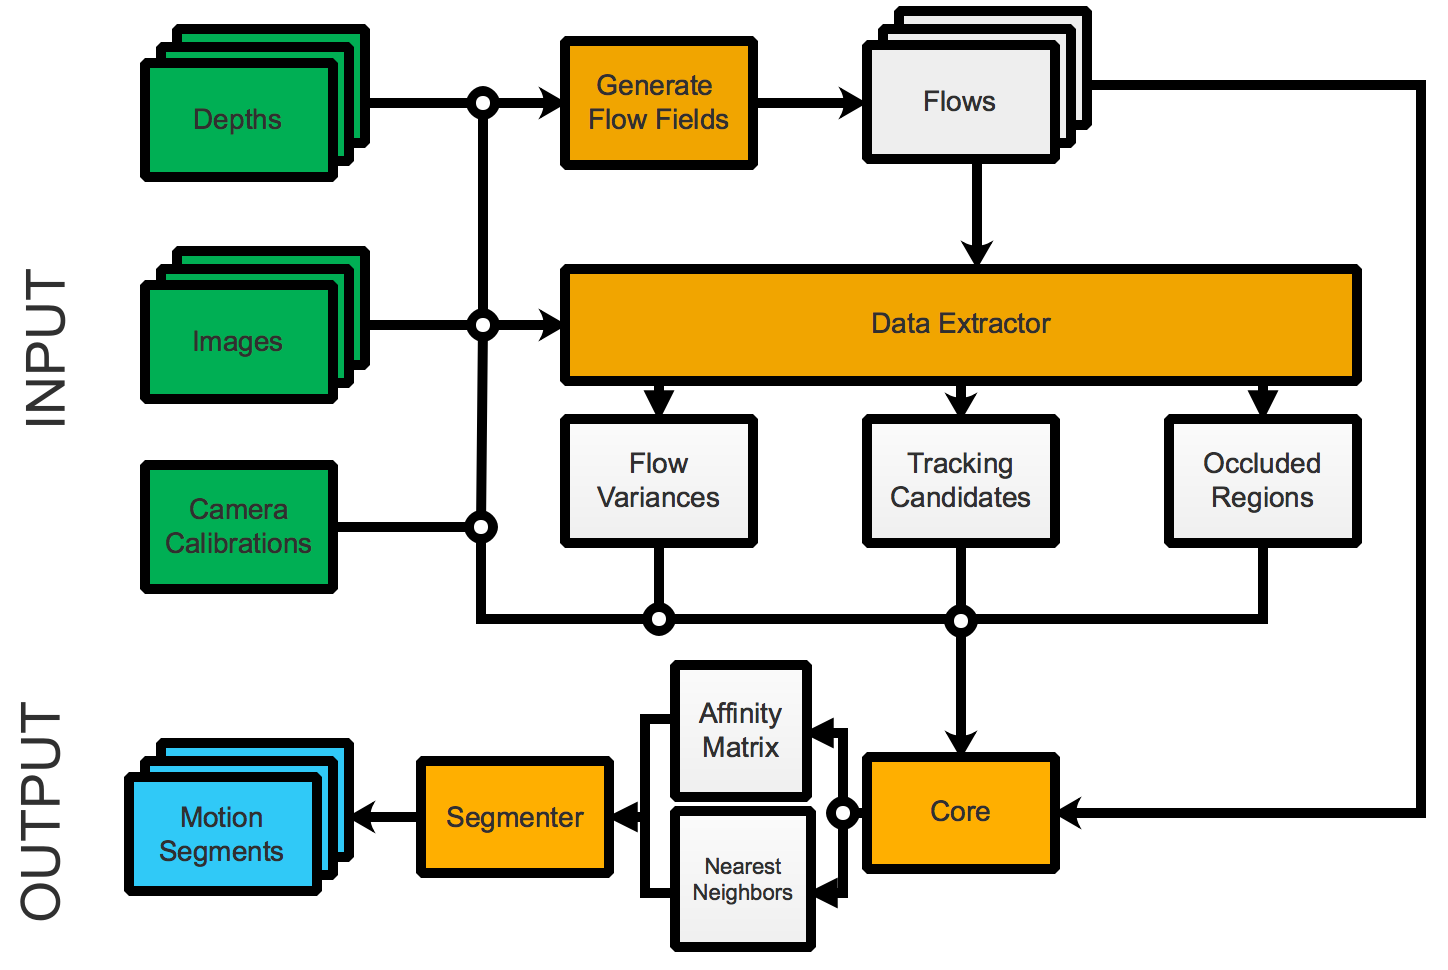
\includegraphics[width=0.9\linewidth] {implementation/pipeline}
\end{center}
\caption[Motion Segmentation Pipeline]{A schematic illustration of the structure of our pipeline. Individual pipeline components are drawn as orange boxes. The initial input is drawn as green boxes, the resulting final output as a blue box. Intermediate outputs are drawn as gray boxes. The arrows indicate the data-flow, whereas the white dots indicate a data-flow multiplexing. That means, data that flows through such a dot is used by several pipeline components.}
\label{fig:pipeline_schematic}
\end{figure}
In the following let us briefly outline the main stages of our motion segmentation pipeline, which is additionally visualized in figure $\ref{fig:pipeline_schematic}$:
\begin{enumerate}
\item \textbf{Dataset Preparations} (Sec. $\ref{sec:dataset_preparations}$): Initially, the frames and depth maps of a given RGB-D video have to be extracted and named according to our pipeline naming conventions. Moreover, the depth map range is normalized to be in meter units.
\item \textbf{Generate Optical Flows} (Sec. $\ref{sec:generate_of}$): Next, the forward- and backward-flows on the input sequence is computed.
\item \textbf{Data Extractor} (Sec. $\ref{sec:data_extraction}$): During t
In this stage we extract traceable feature locations in our images. Also, a mask containing all invalid tracking locations per image is computed by checking whether the the forward and backward flow correspond to each other. Optionally, depth data, flow and depth variances and color maps are extracted that are used within a later pipeline stage. 
\item \textbf{Trajectory Tracking} (Sec. $\ref{sec:trajectory_tracking}$): The previously computed flows are used to perform a point tracking on the extracted traceable features. The ordered sequence of tracking points of a feature is called trajectory.
\item \textbf{Affinity Matrix Generation} (Sec. $\ref{sec:affinity_matrix_impl}$): In this stage the similarities between all trajectory pairs are computed. This is achieved by computing the color-, spatial- and motion distance between the overlapping segments of a pair and combining them in a certain way.
\item \textbf{Segmenter}: Our pipeline offer two types of segmentations, sparse and dense segmentations. 
	\begin{enumerate}
	\item \textbf{Sparse Motion Segmentation} (Sec. $\ref{sec:sparse_motion_segmentation}$): Using the affinity matrix plus the nearest neighbouring trajectories per trajectory, we can compute its dense segmentation by either applying a spectral clustering on the affinity matrix or by reformulating the problem as a graph cut problem. Usually
	\item \textbf{Dense Segmentation} (Sec. $\ref{sec:dense_motion_segmentation}$): Optionally, our pipeline allows to transform the sparse segmentation into a dense segmentation. 	
	\end{enumerate}
\end{enumerate}
In the following sections we examine and discuss each individual pipeline stage in detail. 

\section{Dataset Preparations}
\label{sec:dataset_preparations}
The preparation of an input datasets is the very first stage of our pipeline. Initially, we have to either capture a video using one of our capturing devices or use an existing video sequence. Next, we extract all the frames from the considered video. In case there are also depth maps$\footnote{In case we are working with depth data, we assume that there exists one depth map per frame. Our pipeline assumes, that the values in the depth images are in meter units}$ available, they are transformed such that their value range is in meter units. An example of a color frame and its depth field is shown in figure $\ref{fig:color_and_depth_image}$.
\begin{figure}[H]
\begin{center}
\subfigure[Color Frame]{
   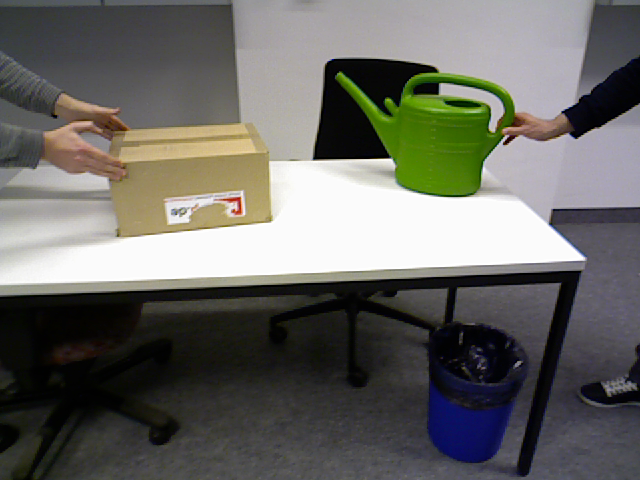
\includegraphics[width=0.48\linewidth] {implementation/preproc/18}
   \label{fig:color_and_depth_image_a}
}
\subfigure[Depth Field]{
   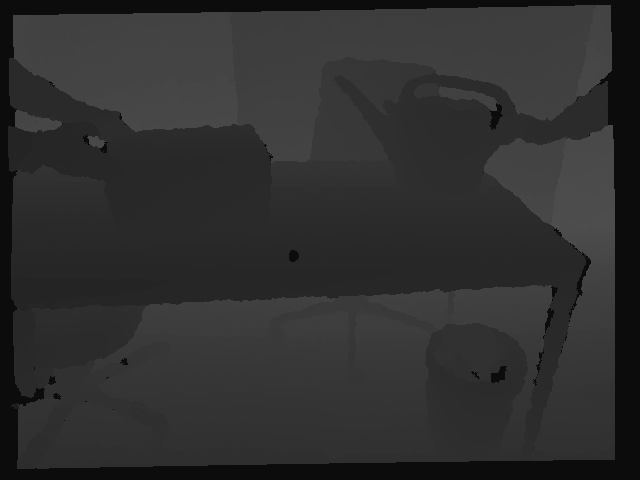
\includegraphics[width=0.48\linewidth] {implementation/preproc/depth_18}
   \label{fig:color_and_depth_image_b}
}
\end{center}
\caption[Color and Depth Image]{An example of a color image / depth field pair.}
\label{fig:color_and_depth_image}
\end{figure}
A depth filed has the same name as its corresponding video frame. Moreover, our pipeline assumes a well-enumeration of its video frames, meaning that the frame, which corresponds to the $k-th$ frame is referenced by the name \textit{k}. \\ \\
A listing of our datasets can be fond in section~\ref{sec:datasets} on page~\pageref{sec:datasets}. \\ \\

\section{Generate Optical Flows}
\label{sec:generate_of}
In our pipeline we heavily rely on optical flow fields. In particular, flow fields are used to perform the point tracking to extract motion trajectories, to detect occlusions and for computing the affinities between trajectories. Therefore, the quality of the flow fields highly affects the final outcome of the motion segmentation. \\ \\
A conceptual idea as well as a mathematical formulation of optical flow fields is provided in section $\ref{sec:optical_flow}$ on page $\pageref{sec:optical_flow}$. However, in principle, the optical flow represents a displacement field that defines where a certain point in a frame is mapped to in its successor frame. \\ \\
In this stage we want to generate the following optical flows on the frames of given dataset video:
\begin{itemize}
	\item The \textbf{forward flow} fields: Refers to the optical flow between a frame and its successor frame.
	\item The \textbf{backward flow} fields: Refers to the optical flow between a frame and its predecessor frame.
\end{itemize}
For the actual computation of the optical flows we rely on existing implementations. In particular we use the freely available implementations of the methods discussed in section $\ref{sec:optical_flow}$ on page $\pageref{sec:optical_flow}$. In the following a short list of the flows integrated in our pipelines and their main properties:
\begin{itemize}
\item The enhanced version of the original flow method proposed by Horn and Schunck (\textbf{HS}): This flow estimation method is a tweaked version of H.S. original formulation. The authors offer a freely available Matlab implementation that has a decent run-time. Please note that this implementation does not make use of depth maps to compute the flow estimations.
	\begin{itemize}
	\item Simple formulation and fast to run.
	\item Matlab implementation freely available.
	\item Does not make use of depth fields.
	\end{itemize}
\item The large displacement optical flow estimation (\textbf{LDOF}): LDOF implements a flow estimation method that is capable to handle large motions and thus yields a better quality fast moving objects flow estimates. This method, however, does also not make use of depth fields. The authors offer a freely available, compiled C++ program. The program has an intermediate runtime of about 30 seconds per $480 \times 640$ pixel frame.
	\begin{itemize}
	\item Can handle large displacements, i.e. fast moving objects.
	\item Compiled C program freely available
	\item Does not make use of depth fields
	\end{itemize}
\item The Semi-rigid scene flow (\textbf{SRSF}) method: The authors offer a partially available code basis that can be compiled to a executable program. The program can only generate motion segmentations for dataset that have a image resolution of 480 by 640 pixels. Since the program makes use of depth fields, corresponding depth maps have to be provided in the pipeline's formatting conventions. A detailed descriptions about their pipeline conventions can be found in their documentation$\footnote{See \url{http://lmb.informatik.uni-freiburg.de/Publications/2014/Bro14/}}$. 
	\begin{itemize}
	\item Makes use of depth maps: formulates a local and global motion by jointly using intensity and depth data.
	\item Models motion as a global rigid motion plus a non-rigid residual
	\item Free C++ code availbe, some parts are only available as binaries.
	\item Can only be run on videos with a resolution of 640 by 480 pixels
	\end{itemize}
	
	
	They regularize the flow field in this 6-DoF parametrization such that their model favors lo- cally rigid motions.
	solve for the local and global motion by jointly using intensity and depth data
the model the scene flow as a 3d vector field consisting of a global rigid motion plus a non-rigid residual

	
	
\item The Layered RGBD flow (\textbf{LRGB}) method: The LRGBD method segments motion into layers ordered according to the depth ranking. The authors offer a freely available Matlab implementation which takes about 10 minutes per 640 x 480 pixel frame to compute its forward and backward flow.
	\begin{itemize}
	\item Makes use of depths to handle occlusions
	\item Layered RGBD scene flow estimation method
	\item Very slow in terms of computation time
	\item They offer a freely available Matlab implementation
	\end{itemize}
\end{itemize}
For the reminder of this thesis let us use the abbreviations defined in the list above when referring to a particular flow method. \\ \\
Lastly, figure $\ref{fig:flow_method_flows}$ shows an example output produced by running these method on a common frame:
\begin{figure}[H]
\begin{center}
\subfigure[HS]{
   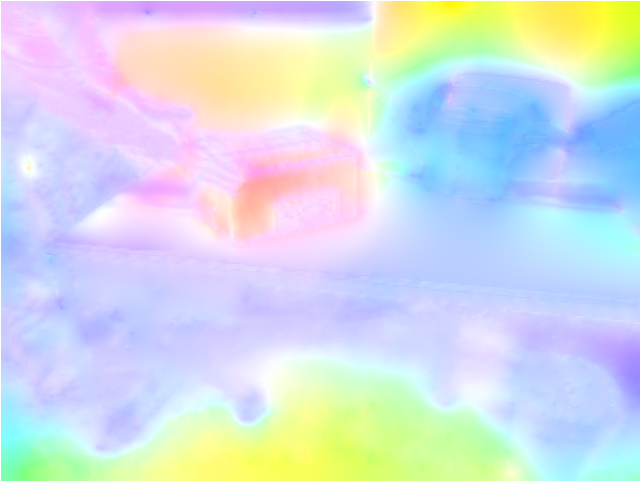
\includegraphics[width=0.47\linewidth] {implementation/flow_methods/hs}
   \label{fig:flow_method_flows_a}
}
\subfigure[LDOF]{
   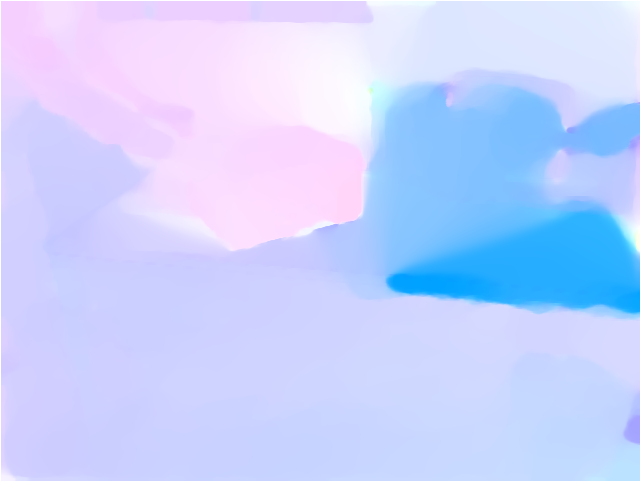
\includegraphics[width=0.47\linewidth] {implementation/flow_methods/ldof}
   \label{fig:flow_method_flows_b}
}
~
\subfigure[LRGBD]{
   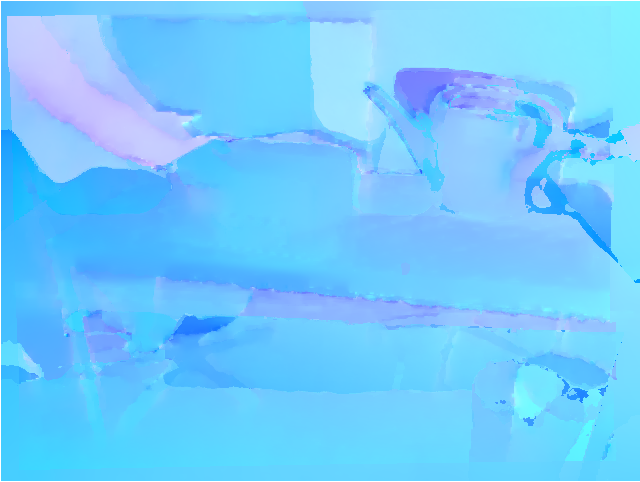
\includegraphics[width=0.47\linewidth] {implementation/flow_methods/lrgbd}
   \label{fig:flow_method_flows_c}
}
\subfigure[SRSF]{
   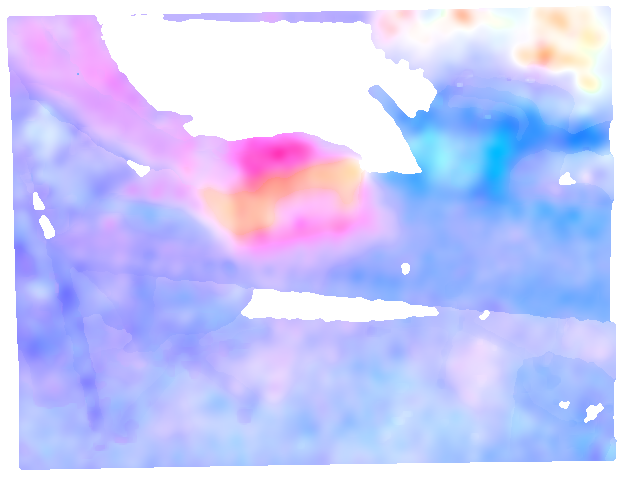
\includegraphics[width=0.47\linewidth] {implementation/flow_methods/srsf}
   \label{fig:flow_method_flows_d}
}
\end{center}
\caption[Flow Method Flows]{An visualization of the flow fields produced by our used flow methods when running them on the same frame sequence. Please notice that the color encoding is the same as introduce in section $\ref{sec:optical_flow}$ on page $\pageref{sec:optical_flow}$.}
\label{fig:flow_method_flows}
\end{figure}

\section{Data Extraction}
\label{sec:data_extraction}
In this section we offer the reader a detailed description of what data and how it is extracted. This pipeline stage can be understood as a pre-processing stage. \\ \\
In particular we will explain how meaningful image locations of moving objects are determined, how we detect occlusions and lastly we develop a technique to normalize the flow fields which enables us to dump the influence of erroneous flows. Algorithm $\ref{alg:data_extraction}$ gives an overview of the involved steps in this stage.
\begin{algorithm}[H]
\caption{Data Extraction}
\begin{table}[H]
  \begin{tabular}{@{}lll@{}}
    \textbf{Input:} & Dataset Images \bf{F} \\
		& Forward- and Backward Optical Flows \bf{OF} \\
 		& Depth Images (\emph{optional}) \bf{DI} \\
    \textbf{Output:} & Traceable Feature Locations \bf{TF} \\
    & Occluded Location Masks \bf{OM}\\
    & Cie-Lab Color Images \bf{CI} \\
    & Flow Variances \bf{FV} \\
    & Depth Variances \bf{DV} \\
    
  \end{tabular} 
\end{table}
\setlength{\fboxrule}{0pt} 
\begin{boxedminipage}{1.0\textwidth}
  \begin{algorithmic}[1]
      \ForAll{$\text{frame } f \in \bf{F}$}
        \State $\text{Run Thresholded Harris Corner Detector}.$
		\State $\text{Append Sampled Features to } \bf{TF}.$
		\State $\text{Fetch } fwf,bwf \in \bf{OF} \text{ that belongs to f}.$
		\State $\text{Apply forward-backward-flow check on fwf and bwf} \bf{TF}.$
		\State $\text{Append invalid check locations to } \bf{OM}.$
		\State $\text{Apply a special variant of the bilateral filter on fwf}.$
		\State $\text{Append filtered flow to } \bf{FV}.$
		\State $\text{Transform f to CIE Lab Colorspace and append it to } \bf{CI}.$
		\State $\text{Fetch } df \in \bf{DI} \text{ that belongs to f}.$
		\State $\text{Apply a 2-pass special variant of the bilateral filter on } df$
		\State $\text{Append the filtered depth to } \bf{DV}$
      \EndFor
  \end{algorithmic}
  \end{boxedminipage}
  \vskip1.5pt
\label{alg:data_extraction}
\end{algorithm}
For every dataset frame we extract potential tracking candidate, the forward-and backward flow to the next frame, the occlusion map and colors in the CIE lab space, the normalized depth fields ranging in meter units and the depth-and flow variances. All this data is then saved to an individual file and used in a later pipeline stage.
\subsection{Tracking Candidates}
\label{sec:tracking_candidates}
In this section we explain our approach how we determine image locations that exhibit meaningful motion information and thus are good candidates to track. The found tracking candidates are later used as the staring position by our point tracker and thus responsible for detecting moving objects. \\ \\
Our implementation determines moving object regions by performing a grouping on motion trajectories. However, to form such trajectories we need to run a tracing on reliable motion features over the given video sequence. So, what are these features and how are they detected? \\ \\
In this section we therefore explain how to determine reliable and meaningful image locations that exhibit motion information and thus are good candidates to track. The found tracking candidates are later used as the staring position to trace features. Therefore, the quality of the candidates affects the detection of the moving objects. \\ \\
The simplest idea would be to simply track every pixel location. On one hand, this would indeed capture every moving object. On the other hand, however, this also would make the motion tracking task highly inefficient, yet infeasible for common image resolutions. Therefore, we want a method which offers us a sparse sampling of the image locations but the same time hits enough meaningful candidates. \\ \\
Ideally, we want to use a feature detector that ignores points in homogeneous areas but selects points that show structural information in their vicinity. Since image corners exhibit a lot of structural information a Harris detector is a solid choice to approach this task. \\ \\
The idea of this detector is the following: A corner defines an intersection of two edges. Therefore, it represents a point in which the directions of these two edges change. For images this means that the gradient has a large variance at that location. \\ \\
It is possible to describe the average intensity change in any direction $(x,y)$
as a bilinear from
\begin{equation}
\left( x,y \right) M \colvec{x}{y}	
\end{equation}
Within the Harris detector code, every image location is then described in terms of the eigenvalues of $M$. Moreover, the detector uses the pixel-wise eigenvectors to measure the corner response. Good corners have a large intensity change in all directions thus their measured response should be large and positive. A detailed formulation of the Harris corner detector can be found in section $\ref{sec:harris_corner_detector}$ on page $\pageref{sec:harris_corner_detector}$. \\ \\
We apply the described Harris corner detector on every dataset image. This procedure yields a sparse set of traceable corner candidates per frame. Additionally, candidates with a too weak corner response are filtered according to a certain threshold value. This ensures to only track strong edges and reliable features. \\ \\
Lastly, for efficiency reasons, we spatially subsample the extracted locations. The subsampling is performed by applying a boolean grid with a certain cell size on the candidates, which acts as a selection mask. This reduces the number of tracking candidates drastically and makes the sampling even more sparse. Hence, we have to track fewer features and the overall runtime decreases. \\ \\
The image locations of the remaining candidates are then dumped into a file. An example of this tracking candidate extraction procedure is illustrated in figure $\ref{fig:tracable_candidates}$. \\ \\
\begin{figure}[H]
\begin{center}
\subfigure[Input Image]{
   \includegraphics[width=0.48\linewidth] {implementation/candidates/01}
   \label{fig:c14_f1_cand}
}
\subfigure[Sparse Candidates]{
   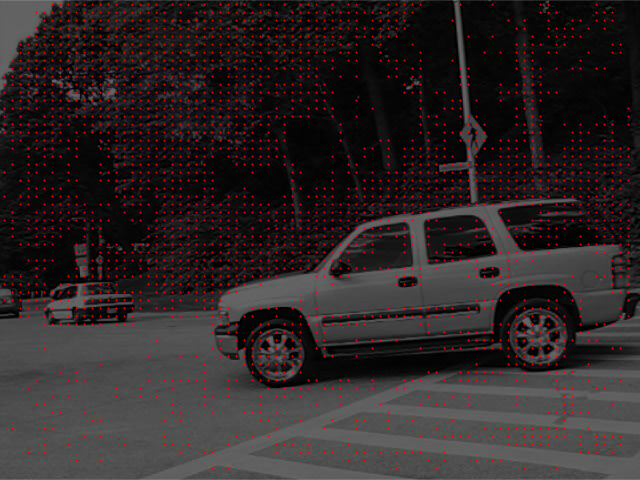
\includegraphics[width=0.48\linewidth] {implementation/candidates/candidates_sparse}
   \label{fig:c14_cand_sparse}
}
~
\subfigure[Harris Corners]{
   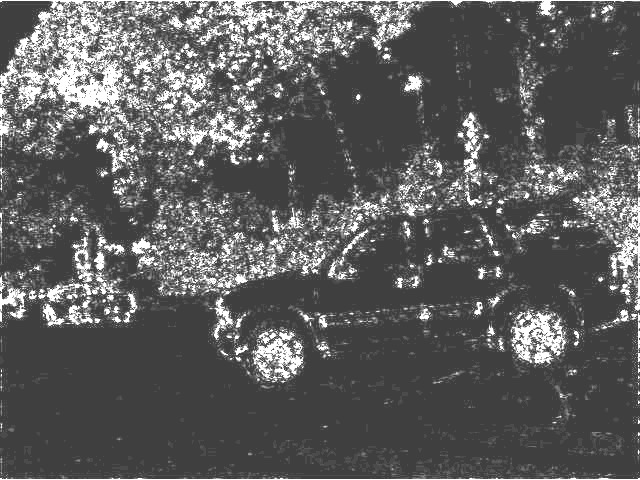
\includegraphics[width=0.48\linewidth] {implementation/candidates/out_corners}
   \label{fig:c14_cand_corners}
}
\subfigure[Dense Candidates]{
   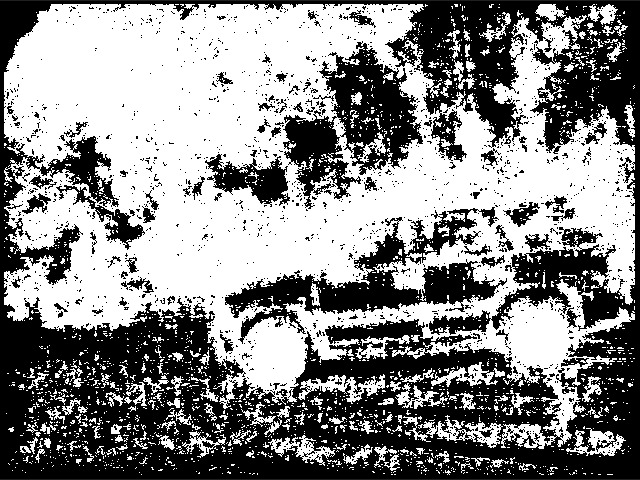
\includegraphics[width=0.48\linewidth] {implementation/candidates/c14_f1_candidates}
   \label{fig:c14_cand_dense}
}
\end{center}
\caption[Tracking Candidates]{A visualization of the tracking candidates extraction stages. For a given input image as shown in subfigure $\ref{fig:c14_f1_cand}$ we want to compute a sparse set of traceable feature locations as shown in subfigure $\ref{fig:c14_cand_sparse}$. The candidates are visualized as a boolean matrix for which true means a valid traceable candidate and false an invalid tracking location.}
\label{fig:tracable_candidates}
\end{figure}
For any given dataset frame (fig. $\ref{fig:c14_f1_cand}$) we compute its corners (fig. $\ref{fig:c14_cand_sparse}$) by applying a Harris corner detector. By thresholding the resulting corners we reject too week candidates and thus obtain a dense sampling of candidate locations (fig. $\ref{fig:c14_cand_dense}$). Lastly, by subsampling the candidates, we further can reduce their number and obtain the final sparse list of candidates (fig. $\ref{fig:c14_cand_sparse}$). \\ \\
So, the remaining question is: What grid size should be used to generate the sparse set of tracking candidates? To answer this question we run different sampling rates on the tracking candidates and evaluated which size was able to produced the best motion segmentations. An visualization of tracking candidates produced by using different sampling rates is shown in figure $\ref{fig:sampling_rate_candidates}$. 
\begin{figure}[H]
\begin{center}
\subfigure[Extreme Oversampling]{
   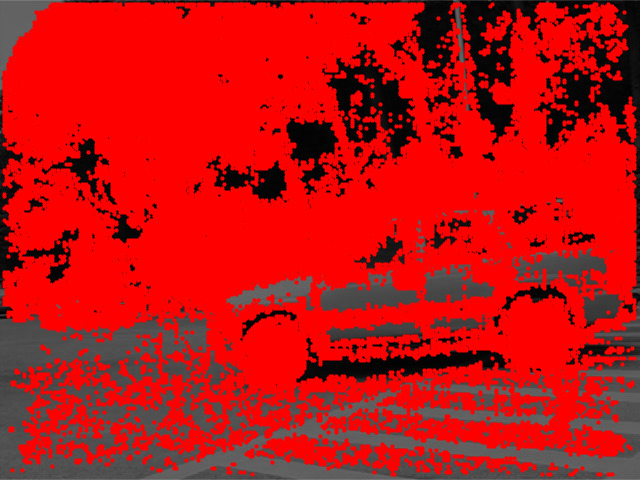
\includegraphics[width=0.48\linewidth] {implementation/candidates/sr_2}
   \label{fig:c14_extreme_oversampling}
}
\subfigure[Oversampling]{
   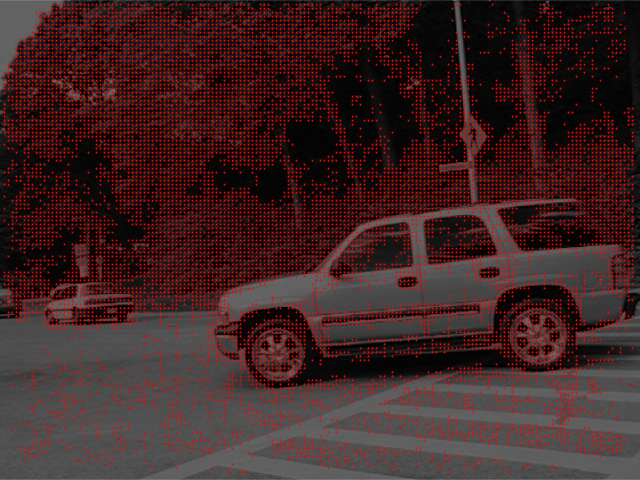
\includegraphics[width=0.48\linewidth] {implementation/candidates/sr_4}
   \label{fig:c14_oversampling}
}
~
\subfigure[Ideal Sampling Rate]{
   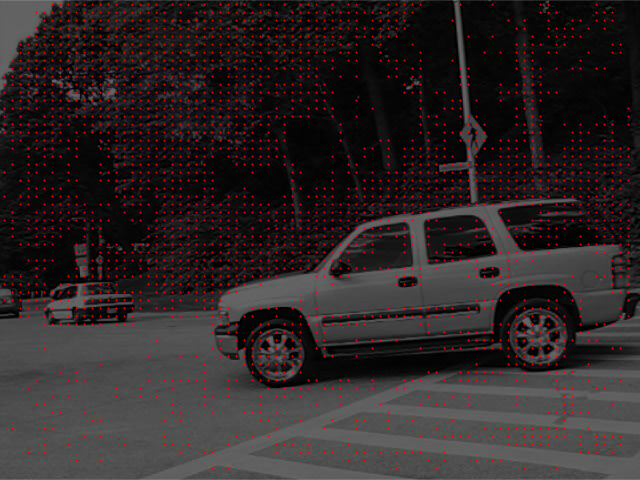
\includegraphics[width=0.48\linewidth] {implementation/candidates/sr_8}
   \label{fig:c14_ideal_sampling}
}
\subfigure[Undersampling]{
   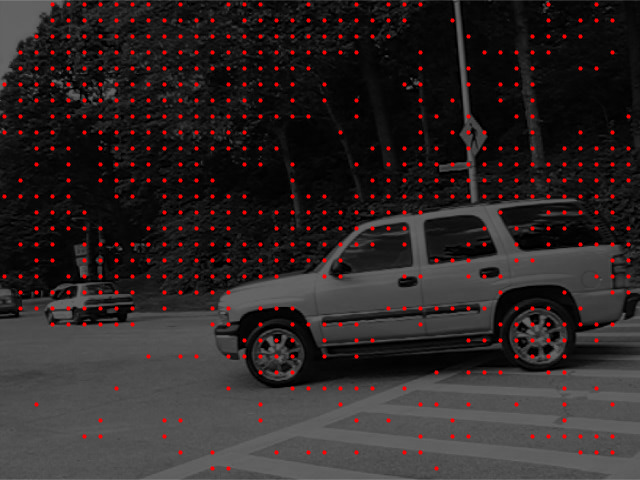
\includegraphics[width=0.48\linewidth] {implementation/candidates/sr_16}
   \label{fig:c14_undersampling}
}
\end{center}
\caption[Density Of Candidates For Different Sampling Rates]{A visualization of different sampling rates of tracking candidates}
\label{fig:sampling_rate_candidates}
\end{figure}
After tinkering with this parameter during our experiments we observed, that setting the cell size larger than 12 pixels causes a lose in detail since there are not enough points to cover small object parts. On the other hand, cells smaller than 6 pixels waste computation time as smaller objects tend to get smoothed away. Hence, our pipeline samples every 8th pixel by default. However, please note that it is still possible to manually assign a different value to this parameter. \\ \\
Finally, there is one optional post-processing stage, which removes all candidates that map to a too weak optical flow vector. This reduction is implemented as the follows: We use the tracking candidate of a frame as lookup coordinates in their corresponding forward flow fields and compute their magnitude. Then, every candidate that maps to a magnitude value smaller than the largest 10 percent of the determined flow magnitudes is discarded. We repeat this procedure for every frame. Doing so drastically reduced the total number of candidates. However this procedure may also cancel out useful motion locations. Nevertheless, most of the time this post-processing only removes candidates that belong to the background$\footnote{By \textit{background} we refer to pixel locations that do not map to a moving object.}$. Additionally, figure $\ref{fig:tracable_candidates_strict}$ graphically illustrates the idea behind this filtering approach.
\begin{figure}[H]
\begin{center}
\subfigure[Subselection of all Dense Candidates]{
   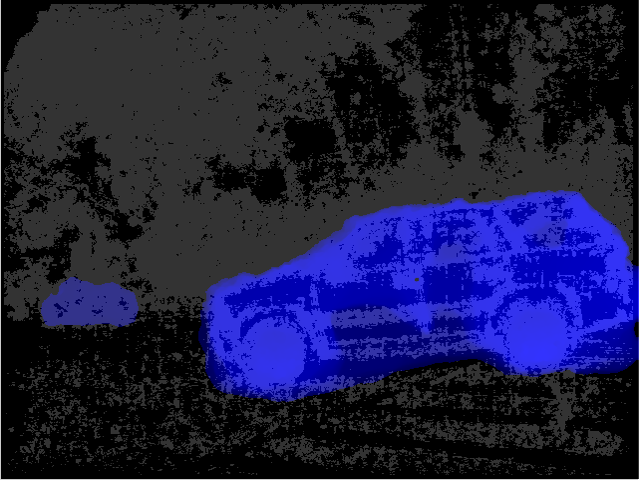
\includegraphics[width=0.48\linewidth] {implementation/candidates/subsel_flow_mags}
   \label{fig:c14_f1_cand_dense_2}
}
\subfigure[Strict Dense Candidates]{
   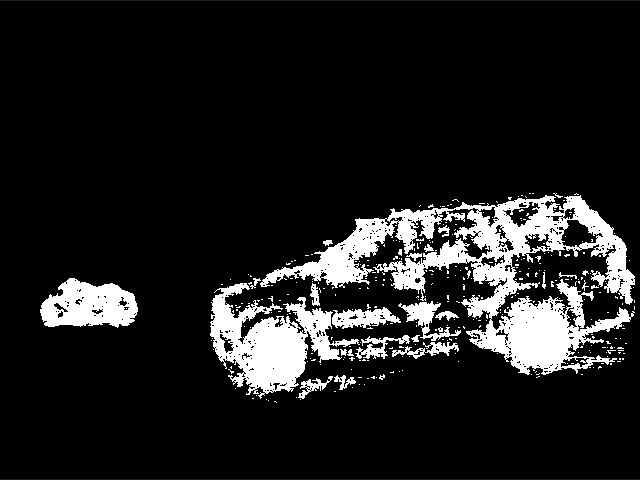
\includegraphics[width=0.48\linewidth] {implementation/candidates/strict_dense_candidates}
   \label{fig:c14_cand_dense_strict}
}
\end{center}
\caption[Strict Dense Candidates]{A visualization of the post-processed traceable candidate locations. On the left, all extracted candidate locations overlaid by the flow magnitudes (in blue), on the right side, an image of the reduced candidates.}
\label{fig:tracable_candidates_strict}
\end{figure}
In the image on the left (fig. $\ref{fig:c14_f1_cand_dense_2}$) we see the set of all dense tracking candidates overlaid by their flow magnitudes (the bluish masks). The stronger the magnitude, the more bluish the mask is colored. We trivially observe, that the moving objects themselves correspond to the top flow magnitudes. Hence, applying a filtering the tracking candidates by their flow magnitudes yields tracking candidates on the moving objects (fig. $\ref{fig:c14_cand_dense_strict}$). \\ \\
Both moving objects in the shown example are preserved and only background pixels are removed. However, keep in mind that this post-processing may filter small, meaningful motions. Especially, when there is a lot of camera motion involved, this approach may fail. \\ \\
Up to this moment we know \textit{when} (i.e. in what frame) and \textit{where} (i.e. at which location) we have to \textit{start} trajectories while running our point tracker. Moreover, by using the forward flows we know where the extracted features have to be tracked to in their successor frame. However, what we still do not know is \textit{when to end} the tracking of a trajectory. Usually, a trajectory is supposed to end when it gets occluded by an obstacle. In the next section we discus how to find occluded regions.

\subsection{Occlusion detection}
\label{sec:occlusion_det}
In this section we discuss how to determine when we should stop tracking a particular tracking candidate. This is particularly important since otherwise groupings on motion trajectories would be very erroneous and thus would negatively affect the motion segmentation quality. \\ \\
The previously determined tracking candidates are used as starting points for out point tracking. For every tracking candidate we determine its tracked to position by adding the appropriate forward flow. However, this approach is very error prone because of using incorrect flow estimations or occluded regions. \\ \\
Occlusion may occur whenever a previously visible object gets covered by another object. For instance when a object close to a camera gets directly in front of an object in the background. Continuing to trace a occluded point yields an incorrect tracking, since two distinct objects are tracked by the same trajectory. Thus, we have to stop tracking points as soon as they get occluded.
\begin{figure}[H]
\begin{center}
\subfigure[Input Image]{
   \includegraphics[width=0.48\linewidth] {implementation/occlusion/01}
   \label{fig:c14_f1_occ}
}
\subfigure[Occluded Regions]{
   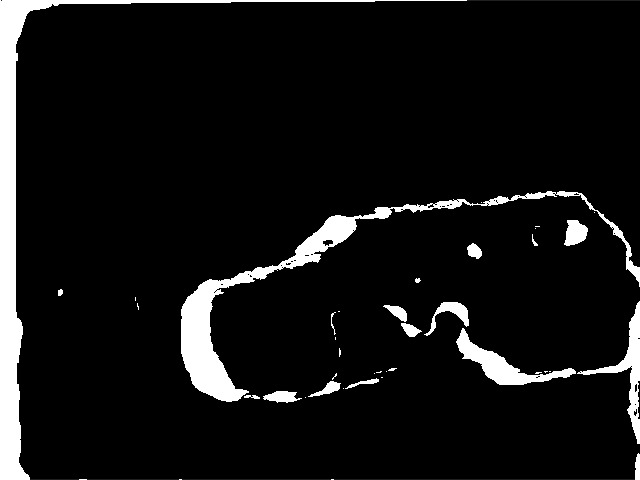
\includegraphics[width=0.48\linewidth] {implementation/occlusion/invalid_regsions}
   \label{fig:c14_invalid_regions}
}
\end{center}
\caption[Occluded Regions]{A visualization of occluded regions. On the left, an color video frame and on the right its corresponding occluded regions (white pixels).}
\label{fig:invalid_regions}
\end{figure}
In tracking tasks, occlusion is usually detected by comparing the appearance of the local neighborhood of the tracked point over time. In contrast, we detect occlusions by verifying a consistency check between the forward- and backward flows. Such a verification is performed by applying the backward flow $\hat{w}_t$ to its continued tracked point $p_{t+1}$ and then checking whether the resulting point has the same origin $\hat{p}_t$ as the actual tracked from position $p_t$. Additionally, we visually outlined this concept of occlusion detection in figure $\ref{fig:occlusion_detection}$. Moreover, an example of occluded regions produced by following our approach is shown in figure $\ref{fig:invalid_regions}$ shows an of a generated occlusion.
\begin{figure}[H]
\begin{center}
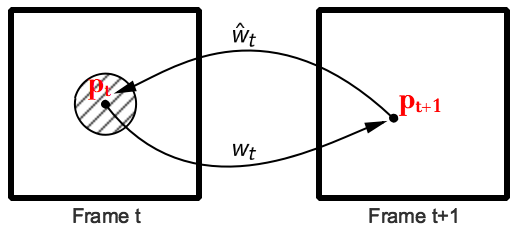
\includegraphics[width=0.6\linewidth] {implementation/occlusion/occ_det}
\end{center}
\caption[Occlusion Detection]{Conceptual illustration of occlusion detection. For any tracking candidate we apply its corresponding forward flow to find its position in the next frame. From there, we look-up its backward flow and apply it on the tracked to position. If we land close to the point in the original tracked from frame, we say, that the point is not occluded and otherwise we call the point occluded.}
\label{fig:occlusion_detection}
\end{figure}
In the non-occluded case, the backward flow vector $\hat{w}_t$ is supposed to point to the inverse direction of its corresponding forward flow vector $w_t$. Hence, adding $w_t$ to the backward flow vector looked up at the location the forward vector points to should yield approximately the zero vector. If this required consistency is not satisfied, then the point $p_t$ is either getting occluded at frame $t+1$ (the next frame) or the flow was not correctly estimated. Both outcomes are good reasons to stop tracking this point at frame $t$. Since there are always some small estimation errors in the optical flow, there is a small tolerance interval granted. The formula used to decide when a point is not occluded is given in equation $\ref{eq:occlussion_error_tol}$.
\begin{equation}
\begin{aligned}
& \forall p_t \in \text{Frame t}:	\norm{\hat{p_t}-p_t}_2^2 < \epsilon \norm{\hat{w}_t + w_t}_2^2 + b \\
& \text{where } \hat{p_t} = p_{t+1} + \hat{w_t} \text{ with } p_{t+1} = p_t + w_t
\end{aligned}
\label{eq:occlussion_error_tol}
\end{equation}
Whenever a trajectory got occluded then this also means that an new moving object appeared. In that case the occluded regions represent empty areas yet not covered by any trajectories that belong to the occluding objects. Hence, in every such empty area, new trajectories are initialized. This urge of having to starting new trajectories in occluded regions is also known as \textit{disocclision}.

\subsection{Flow Variance}
\label{sec:flow_variance}
So far, we were assuming that the generated flow fields are good estimates in as sense that they do not exhibit an enormous amount of noise. However, especially along motion boundaries, this assumption is very dangerous. For instance, when taking the difference between two noisy flow vectors, then the noise level can get amplified on the resulting vector. This is especially problematic while computing similarities between trajectories based on the motion distance. In that case, utilizing repeatedly noisy flow differences will negatively affect resulting segmentation quality. \\ \\
In this section we therefore propose a normalization factor that reduces the influence of potential noise present in the estimated flow fields. A simple, first idea would be to smooth the flows by applying a low-pass filter$\footnote{The purpose of a low pass filter is to damp high frequencies such as noise.}$, such as a Gaussian kernel. On one hand, it surely would reduce the noise level along the motion boundaries, but on the other hand, it also would wash out many relevant motion details. Therefore, filtering the flows directly is not recommendable and we instead would like to follow another, more robust idea. \\ \\
The rationale behind our approach is that the variance on the weights of a low-pass filter are a reliable local indicator for the strength of noise and thus may be used to damp flows differences. \\ \\
Another prominent low-pass filter is the Bilateral Filter $\textbf{BF}$. Similar to a Gaussian filter, this filter also computes a weighed average of the input, but the same time takes into account the variation of intensities to preserve details, such as edges. In particular, using such a filter would preserve motion boundaries. More details about this filter can be found in the appendix in section $\ref{sec:bilateral_filter}$ on page $\pageref{sec:bilateral_filter}$. \\ \\
So, how could we make use of this filter to implement our idea? Imagine we would know the error of the computed flows. Then, by using the variance of the field, we directly could address the error by normalizing the flow value by its corresponding variance value. However, since we do not know the actual error, we have to formulate a robust flow variance estimator. \\ \\
In the following, let us consider the filter weights $w_{p,q}$ between two pixels $p$ and $q$ in a Bilateral filter defined as in equation $\ref{eq:def_bilateral_filter}$. Furthermore, let $\bf{q}_p$ denote a vector containing all neighbors of pixel $\bf{p}$ and $\bf{w}_p$ stands for the vector containing all weights $w_{p,q}$ between $p$ and its neighbors. Mathematically, this can be formulated as:
\begin{equation}
\begin{aligned}
& \bf{q_p} = \left( q_1, \dots, q_{|\mathcal{N}_p|} \right) \\
& \bf{w_p} = \left( w_{p, q_1}, \dots, w_{p, q_{|\mathcal{N}_p|}} \right) \\
& \text{where } \forall q_k \in \mathcal{N}_p
\end{aligned}
\label{eq:bilat_weight_components}
\end{equation}
The definitions from equation $\ref{eq:bilat_weight_components}$ enable us to estimate an expected value of pixel $\bf{p}$ defined as
\begin{equation}
	\mathbf{E} \left[ \bf{p} \right] = \frac{\bf{w}_{p}^{T} \bf{q}_p}{\norm{\bf{w}_{p}}}
\end{equation}
For a given optical flow $\bf{F} = (\bf{F_u}, \bf{F_v})$ we then can estimate its variance by the definition stated in equation $\ref{eq:flow_var_opt_flow}$.
\begin{equation}
	\mathbf{Var} \left[ \bf{F} \right] = \frac{1}{2} \left( \mathbf{Var} \left[ \bf{F_u} \right] + \mathbf{Var} \left[ \bf{F_v} \right] \right)
\label{eq:flow_var_opt_flow}	
\end{equation}
So, it turns out that the flow variance is simple the sum of the variances of the flow directions. Moreover, for estimating the directional component variances we relied on the bilateral filter weights. Practically speaking, we run a Bilateral Filter on the directional scalar fields of any flow field and collected all filter weights. Then we computed the statistics based on the derivations described above. An example of such a variance field for a given flow is shown in figure $\ref{fig:flow_variance}$.
\begin{figure}[H]
\begin{center}
\subfigure[Flow Field]{
   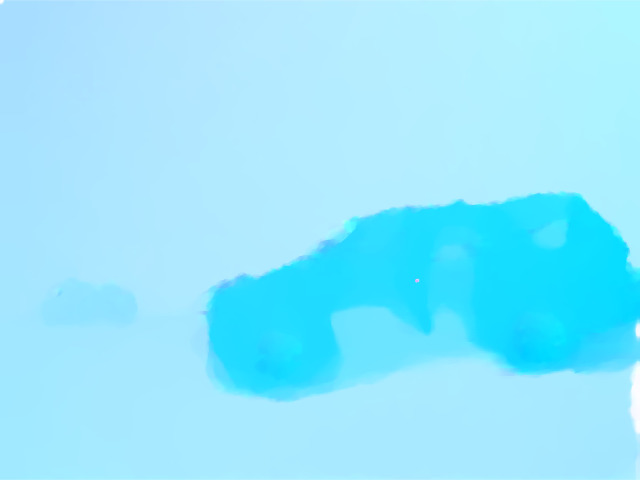
\includegraphics[width=0.48\linewidth] {implementation/flow_var/ff_c14_1}
   \label{fig:c14_fv_flow}
}
\subfigure[Variance Field]{
   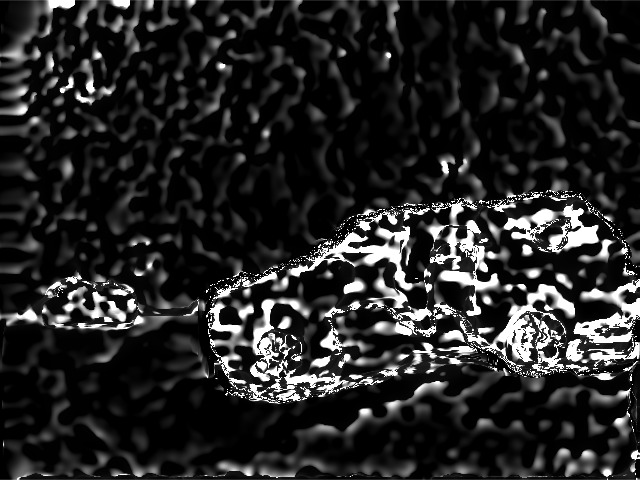
\includegraphics[width=0.48\linewidth] {implementation/flow_var/fv_c14_1}
   \label{fig:c14_fv_var}
}
\end{center}
\caption[Flow Variance]{Visualization of the flow variance computed by applying a bilateral filter on the optical forward flow.}
\label{fig:flow_variance}
\end{figure}
A detailed derivation of equation $\ref{eq:flow_var_opt_flow}$ can be found in the appendix in section $\ref{sec:derivation_flow_var}$ on page $\pageref{sec:derivation_flow_var}$.

\section{Trajectory Tracking}
\label{sec:trajectory_tracking}
As mentioned previously, motion is a spatially and temporally coherent visual cue. This implies that motion is not frame-wise independent and thus it represents the history of every image location. In particular the motion history of a tracking candidate can be formed by tracing them to their successor frames using the optical flow. Another commonly used term for a point history is \textit{motion trajectory}. A trajectory is an ordered list of points produced by tracking an initial feature location over a series of frames. We conclude that every trajectory has a temporal aspect (the frames its tracking points correspond to) and a spatial aspect (the image locations its tracking positions map to). \\ \\
So far we have discussed how to obtain starting positions of trajectories (sec. $\ref{sec:tracking_candidates}$ and when we have to stop them (sec. $\ref{sec:occlusion_det}$). Moreover, by relying on the generated optical flow (sec. $\ref{sec:generate_of}$) we are able to determine the location a point gets tracked to in its successor frame. Therefore, at this moment, we are ready to discuss how to track motion trajectories. \\ \\
In this section we explain in detail the required steps to track motion trajectories. Moreover we discuss a transformation that allows us to obtain 3d world coordinates from the traced 2d trajectory points. For this purpose we will make use of the depth field.

\subsection{Point tracking}
Every point $p_t$ in frame $t$ can be tracked to a position $p_{t+1}$ in its successor frame $t+1$ by using the corresponding forward flow field $w_t$ that belongs to frame $t$. This is achieved by adding $w_t$ to $p_t$, which yields $p_{t+1}$. We repeat this procedure until the points gets either occluded or has reached the last video frame. Algorithm $\ref{alg:point_tracking}$ offers a detailed description of the involved steps to run the point tracking. \\ \\
\begin{algorithm}[H]
\caption{Point Tracking}
\begin{table}[H]
  \begin{tabular}{@{}lll@{}}
    \textbf{Input:} & Tracking candidates \\
    	& Forward Flow fields $\textbf{F}$ \\
        & Occluded Regions \\
	\textbf{Output:} & Trajectories $\textbf{T}$
  \end{tabular} 
\end{table}
\setlength{\fboxrule}{0pt} 
\begin{boxedminipage}{1.0\textwidth}
  \begin{algorithmic}[1]
  	\State $T \leftarrow \text{Initialize an empty list of trajectories}$
  	\State $\bar{T} \leftarrow \text{Initialize an empty list of trajectories}$
  	\For{$k=1 \text{ TO FrameCount}$}
  		\State $C \leftarrow \text{load all tracking candidates that belong to frame } k$
  		\State $\text{Start a new trajectory for each candidate and append it to T}$

  		\ForAll{$\text{Trajectory } t \in T \text{ that has not ended yet}$}
  			\State $p \leftarrow \text{getPointAtFrame(k)}$
  		  	\State $\text{Fetch forward flow vector fv} = \textbf{F} \left(k, p \right)$
  			\State $\text{Compute the tracked to position: } tp = p + fv$
  			\If{$tp \text{ lands in occluded region}$} 
  				\State $\text{End tracking of trajectory } t $
  				\State $\bar{t} \leftarrow \text{Start a new trajectory using tp as starting position}$
  				\State $\text{Append } \bar{t} \text{ to } \bar{T}$
  			\Else 
  				\State $\text{Append tp to trajectory t}$
  			\EndIf
  		\EndFor
  		\State $\text{Move all trajectories in } \bar{T} \text{ to T}$
    \EndFor
  \end{algorithmic}
  \end{boxedminipage}
  \vskip1.5pt
\label{alg:point_tracking}
\end{algorithm}
$\newline$
The point tracker algorithm consists of two main loops. The other loop iterates over the number of frames present in the selected dataset and the inner loop runs over the set of all trajectories. Initially, we load all corner candidates, the occlusion maps and generated flow fields into our pipeline. Then, we initialize an empty trajectory set. \\ \\
In every outer loop iteration we load all tracking candidates that correspond to the current frame index and use them to start new trajectories. Starting a new trajectory by a point means that use that point as the first tracking point of the trajectory plus, we store the frame index of this first point. Moreover, every new started trajectory is marked as not closed, meaning that it can be used to continue its tracking. Only trajectories that were tracked to occluded regions get marked as closed. \\ \\
Next, we proceed with the in the inner loop, which runs the actual point tracking. We select every trajectory that is currently not marked as closed. For each such trajectory we first load its last appended tracking point. Moreover, the flow vector that matches the current trajectory point is loaded. Next, we compute potential tracked to position by addition the forward flow vector to the tracking point. We use the wording \textit{potential}, because we have to check first, whether this point was tracked to an occluded region. \\ \\
In case the point was not occluded we append the computed tracked to position to the trajectory and continue to track the next trajectory. Otherwise, if the point was traced to an occluded region, we have to end the tracking of the currently considered trajectory and mark it as closed. The tracking has to be stopped soon as a point gets occluded, since otherwise the trajectory will share the motion of two different objects. \\ \\
In the occluded case, the computed tracked to position is then used to start a new trajectory. Doing so handles the problem of disocclusion, because empty areas not covered by trajectory yet get filled. \\ \\
This procedure is repeated until we have processed every frame and trajectory. \\ \\
Finally, we conclude this section by offering an example of an actual point tracking applied on the cars dataset. The resulting trajectories, as well as their tracking points, are shown in figure $\ref{fig:cars_trajectories}$. In this visualization we see different trajectories, tracked over four frames. Tracking points that belong to the same trajectory have the same color as their trajectory. As we can see, points that were tracked along the same moving objects exhibit consistent trajectories. In other words, our flow field based tracker produces reliable and meaningful results in this example.
\begin{figure}[H]
\begin{center}

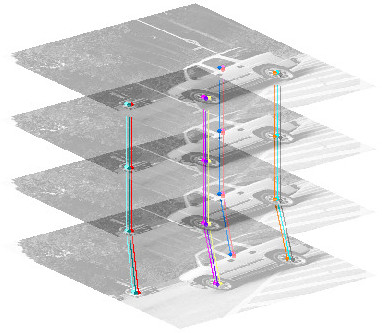
\includegraphics[width=0.65\linewidth] {implementation/trajectories/cars_trajectories_4_sel}
\end{center}
\caption[Trajectories]{Exemplary trajectories tracked in the cars dataset shown in different color. The tracking points exhibit the same color as the trajectory the belong to. The tracking points are plotted as thick dots.}
\label{fig:cars_trajectories}
\end{figure}

\subsection{Transformation to 3d points}
\label{subsection:transform_to_3d_points}
Ultimately, our pipeline should be able to work with 3d data. To enable this, we have to make use of the extracted depth map and use their information in order to transform the 2d trajectory points to 3d points in space. Ideally, the distances, computed to define an affinity measure between trajectories, should be more accurate. 

Given the principal point $p = \left(p_x, p_y \right)$ and the focal lengths $\left(f_x, f_y \right)$ we can compute the following homogeneous transformation:
\begin{equation}
\colvec[f_x X + Z p_x]{f_y Y + Z p_y}{Z} =
\begin{bmatrix}
f_x & 0 & p_x & 0 \\
0 & f_y & p_y & 0 \\
0 & 0 & 1 & 0
\end{bmatrix}
\begin{pmatrix}
X \\
Y \\
Z \\
1
\end{pmatrix}
\end{equation}

In the following, let us assume $d \equiv z$. Then

\begin{equation}
	\colvec[X]{X}{Z} \mapsto \left( \frac{f_x x}{d} + p_x, \frac{f_y y}{d} + p_y \right)^T
\end{equation}

since

\begin{equation}
\begin{aligned}
	d \left( \frac{x - p_x}{f_x} \right) = \hat{x} \Leftrightarrow \frac{\hat{x}}{d} f_x + p_x = x \\
	d \left( \frac{y - p_y}{f_y} \right) = \hat{y} \Leftrightarrow \frac{\hat{y} f_y}{d} + p_y = y 
\end{aligned}
\label{eq:depth_tranfomation}
\end{equation}.
For given pixel coorinates $\left( x,y \right)$ that indicate image locations, we want to transform them into camera coordinates, using depth maps, by applying equation $\ref{eq:depth_tranfomation}$. \\ \\

Given the extrinsic and intrinsic camera calibration data,
\begin{equation}
\begin{aligned}
	\text{Camera}^{depth} : \left( p^d = (p_x^d, p_y^d), f^d = (f_x^d, f_y^d)\right) \\
	\text{Camera}^{color} : \left( p^c = (p_x^c, p_y^c), f^c = (f_x^c, f_y^c)\right) \\
	\textbf{E} : \text{Camera}^{depth} \rightarrow \text{Camera}^{color}
\end{aligned}
\label{eq:calib_data}
\end{equation}.
Steps to transform 2d image locations $\left( u, v \right)$ to 3d positions $\left( x, y, z \right)$ using the camera calibration data defined as in equation $\ref{eq:calib_data}$. Furthermore, let the depth value d $\in$ $\bf{D}$. Then we have to perform the following transformations steps:
\begin{enumerate}
\item Transform image location onto depth camera space
\begin{equation}
	\forall (u, v), \forall d = \textbf{D}(u,v): \colvec[\frac{u - p_x^d}{f_x^d} d]{\frac{v - p_y^d}{f_y^d} d}{d} = \colvec[x]{y}{z} \equiv \bf{p}
\end{equation}
\item Align depth camera on color camera by appling the extrinsic matrix $E$:
\begin{equation}
	\forall p: \hat{p} \equiv \colvec[\hat{x}]{\hat{y}}{\hat{z}} =  E p
\end{equation}
\item transform onto color camera
\begin{equation}
	\forall \hat{p} : \left( \hat{u}, \hat{v}\right) = \colvec{\frac{\hat{x}}{\hat{z}} f_x^c + p_x^c}{\frac{\hat{y}}{\hat{z}} f_y^c + p_y^c}
\end{equation}
\end{enumerate}

\section{Affinity Matrix Generation}
\label{sec:affinity_matrix_impl}
In this section we describe the corresponding pipeline stage that is responsible for generating the so called $\textit{affinity matrix}$, which is later used to compute the actual motion segmentation. For this purpose we compute the pairwise similarities between the previously tracked trajectories according to a certain measure and then use those values to form a similarity graph as defined in section $\ref{sec:similarity_graphs}$ on page $\pageref{sec:similarity_graphs}$. However, computing affinities based on pairwise trajectory distances corresponds to assuming a translational motion model. Especially in real world examples object usually form affine motions $\footnote{An affine motion requires to compute distances on trajectories at a time to verify if it belongs to the a certain motion group.}$ and thus this assumption is imposing a certain error. Despite this limitation we will present a robust solution to this issue. \\ \\
The final affinity matrix correspond to the adjacency matrix representation of the similarity graph. The used metrics are adapted version of the metrics presented in $\cite{OB14b}$ and $\cite{KB15b}$. \\ \\
Generally, trajectories of longer videos are asynchronous, i.e. they cover different temporal windows in a shot. Furthermore, the number of points that are tracked across the whole image sequence is small or even empty due to occlusion, disocclusion or the sampling rate. Hence, a measurement matrix that utilizes the coordinates of the tracked points, as used by the multi-body factorization and subspace methods, will have many missing entries and thus is a bad choice. \\ \\
However, there is a remedy to this issue. We instead compute pairwise affinities between trajectories, because this only requires some trajectories to have some temporal overlap. In particular, we define affinities between all pairs of trajectories that share at least a common frame. \\ \\
According to the gestalt principle of common fate$\footnote{Human tend to group similar objects together that share a common motion.}$, we should assign high affinities to pairs of points that move together. Imagine the situation where two persons are walking next to each other$\footnote{Assume both persons are walking at the same speed in the same direction, ignoring all motions due to deformation.}$. Although they represent different objects, both of them share the same motion. Moreover, person that is sitting stilly in a chair shares the same motion as the objects in the background. The gestalt principle tells us that these situations should be treated conservatively and the objects from these examples should not be separated. \\ \\
In the following we describe in detail the steps of algorithm $\ref{alg:computing_affinity_matrix}$ which is used to generate the affinity matrix.
\begin{algorithm}[H]
\caption{Generating Affinity Matrix}
\begin{table}[H]
  \begin{tabular}{@{}lll@{}}
    \textbf{Input:} & Extracted Trajectories \bf{T} \\
		& Forward Flows \bf{OF} \\
 		& Dataset Images (\emph{optional}) \bf{F} \\
    \textbf{Output:} & Affinity Matrix \bf{W} \\
    & Nearest Trajectory Neighbors \bf{$\mathcal{N}$}\\
    & Trajectory Labels \bf{$\mathcal{L}$}\\
  \end{tabular} 
\end{table}
\setlength{\fboxrule}{0pt} 
\begin{boxedminipage}{1.0\textwidth}
  \begin{algorithmic}[1]
      \State $\text{Form every possible trajectory pair combination of } \bf{T}$
      \State $\text{Filter too short trajectories}$
      \ForAll{$\text{Trajectory pair } \left( \textbf{a}, \textbf{b} \right)$}
        \State $\left( \textbf{p}^a, \textbf{p}^b \right) \longleftarrow\text{Select all temporal overlapping segments between } \textbf{a} \text{ and } \textbf{b}.$
        \State $d_{\text{spatial}} = \text{computeSpatialDistance}\left( \textbf{p}^a, \textbf{p}^b, \textbf{T} \right)$
        \State $d_{\text{color}} = \text{computeColorDistance}\left( \textbf{p}^a, \textbf{p}^b, \textbf{F} \right)$
        \State $d_{\text{motion}} = \text{computeMotionDistance}\left( \textbf{p}^a, \textbf{p}^b, \textbf{F} \right)$
        \State $d^2 = \text{combineDistances} \left( d_{\text{spatial}}, d_{\text{color}}, d_{\text{motion}} \right)$
        \State $W \left( \textbf{a}\text{.label}, \textbf{b}\text{.label} \right) = e^{-\lambda d^2}$
        \State $\text{Update nearest neighbors of } \textbf{a} \text{ and } \textbf{b} \text{ using } d_{\text{spatial}}$
      \EndFor
  \end{algorithmic}
  \end{boxedminipage}
  \vskip1.5pt
\label{alg:computing_affinity_matrix}
\end{algorithm}
As the very first step, our pipeline loads the previously extracted trajectories into its memory. Each loaded trajectory gets a unique identifier, which is called $\textit{label}$, assigned. Next, we discarded every trajectory that is shorter than a user specified threshold to reduce the effect of noisy and invalid tracings. From the remaining trajectories we form every possible pair combination and compute certain distances between them similar as shown in figure $\ref{fig:distance_measure}$.
\begin{figure}[H]
\begin{center}
\subfigure[Overlapping Trajectories]{
   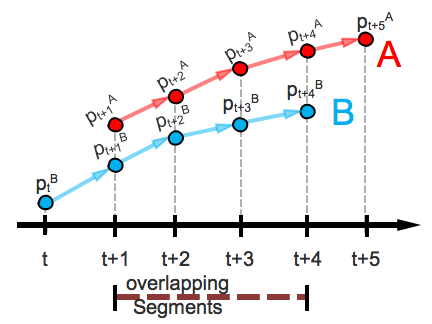
\includegraphics[width=0.7\linewidth] {implementation/affinities/overlapping_tra}
   \label{fig:overlapping_tra}
}
~
\subfigure[Color Distance]{
   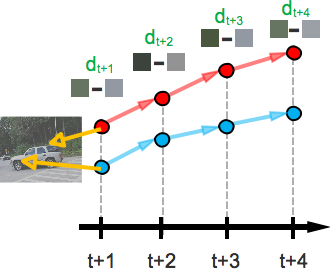
\includegraphics[width=0.3\linewidth] {implementation/affinities/d_co}
   \label{fig:tra_distance_measures_co}
}
\subfigure[Motion Distance]{
   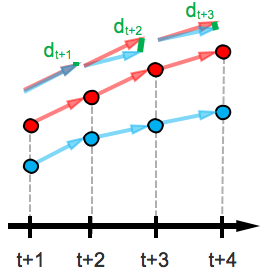
\includegraphics[width=0.3\linewidth] {implementation/affinities/d_mo}
   \label{fig:tra_distance_measures_mo}
}
\subfigure[Spatial Distance]{
   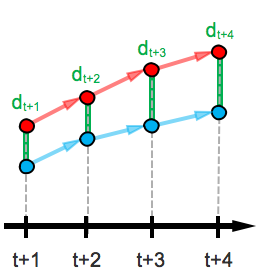
\includegraphics[width=0.3\linewidth] {implementation/affinities/d_sp}
   \label{fig:tra_distance_measures_sp}
}
\end{center}
\caption[Distance Measures]{A graphical example how the mentioned distance metrics can be applied on two trajectories $A$ and $B$. Their $\textbf{spatial distance}$ $d_{\text{spatial}}$ is shown in green, their $\textbf{color distance}$ $d_{\text{color}}$ in orange and their $\textbf{motion distance}$ $d_{\text{motion}}$ in purple.}
\label{fig:distance_measure}
\end{figure}
For any two given trajectories $A$ and $B$ that form a pair, our pipeline computes the following three distances between their temporal overlapping segments$\footnote{By the term \textit{temporal overlapping segments} we refer to tracking point in a trajectory pair that share a common frame.}$:
\begin{itemize}
\item The \textbf{spatial distance} $d_{\text{spatial}}$: Trajectories that belong to the same object are usually spatially close to each other and is defined as
\begin{equation}
	d_{spatial}^{A,B} = \frac{1}{\omega - \alpha + 1} \sum_{k=\alpha}^\omega \norm{A(k) - B(k)}
\label{eq:spatial_distance}	
\end{equation}
where $\alpha$ is the first- and $\omega$ is the last- overlapping frame index between the two given trajectories $A$ and $B$.
\item The \textbf{color distance} $d_{\text{color}}$: Within a certain object region, associated trajectories are tracked at locations that have a similar color value. This distance is defined as
\begin{equation}
	d_{color}^{A,B} = \frac{1}{\omega - \alpha + 1} \sum_{k=\alpha}^\omega \norm{\text{ColorAt}(k, A(k)) - \text{ColorAt}(k, B(k))}_2
	\label{eq:color_dist}
\end{equation}
where $\text{ColorAt}(k, A(k))$ yields a color in CieLab color space$\footnote{Using CieClab colors enables us to use the l2 norm in order to compute color distances.}$ value in frame $k$ at the image location $A(k)$.
\item The \textbf{motion distance} $d_{\text{motion}}$: The rationale of this measure is to exploit$\footnote{Again, thanks to the gestalt principle of common fate we know that for each pair of trajectories at the time instant where their motion is maximally different, the two points do not belong to the same object,}$ the maximal dissimilarity of the two given trajectories via their maximal motion difference among all overlapping frames. The motion distance is defined as
\begin{equation}
	d_{motion}^{A,B}  = \max_t \left( \frac{\norm{\partial_t A - \partial_t B}}{\sigma_t} \right)
\label{eq:motion_distance}
\end{equation}
where the expression $\partial_t A$ denotes the averaged motion over time, which is computed by approximating the derivatives $\partial_t A$, $\partial_t B$ using forward differences with a certain timestep $T$. Furthermore, the resulting motion distance is normalized by its corresponding flow variance value $\sigma_t$. The idea is reduce the influence of noise, which is present in the estimated flow fields. Especially, when taking differences between flow vectors the noise level could get even more amplified. Additional information about this normalization, as well as about the definition of this variance can be found in section $\ref{sec:flow_variance}$ on page $\pageref{sec:flow_variance}$.
\begin{equation}
	\partial_t A = \frac{A(t+T)-A(t)}{T} 
\end{equation}
The exact value of $T$ is the minimum of the number of overlapping frames between the $A$ and $B$ and a fixed threshold. In our pipeline we use $T$ equals 3.
\end{itemize}
where $A(k)$ denotes the tracking position of trajectory $A$ in frame $k$. The final similarity between two trajectories the combination of these distances according to a user-specified combination method. Therefore, let us introduce these combination method that are supported by our pipeline. \\ \\
There are two main setting a user has to specify preliminarily. Whether or not depth cues should be used and how the computed distances should be combined to define an affinity value between trajectories. Both options have a large impact on the final outcome of the affinity matrix. \\ \\
First, when enabling depth cues, all available depth fields are loaded into the pipeline. In combination with the depth- and color-camera calibration data, this enables the pipeline to compute the three dimensional version of each traced trajectory point, analogous as described in the previous subsection $\ref{subsection:transform_to_3d_points}$ on page $\pageref{subsection:transform_to_3d_points}$. As a direct consequence, when using depths, the spatial distance computation is altered. Instead of using the 2d tracking points their 3d transformed versions are used. \\ \\
Furthermore, our pipeline supports two distance combination methods: Either it combines them by calculating the weighted sum of the distance values or it multiplies all the distances. Depending on the used combination strategy, different segmentation methods have to be use later on. Summed distances can only be used in combination together with the $\textit{Kernighan-Lin}$ segmentation method, whereas the product of distances can be either used in our spectral clustering- or min-cut segmentation method$\footnote{The reason for this limitation is due to the fact that the summed distance method may yield negative affinities since some weights are negative.}$. \\ \\
In the beginning of this section, we stated, that our pipeline assumes a translation motion model. This is due to the fact that we compute pairwise distances between trajectory. However, affine motions can locally be approximated by a translation. Therefore, our idea is to damp the effect of model noise by damping the affinities by their spatial distances. The further two trajectories are apart from each other, the less reliable their local approximation is. Both distance combination method will implement this damping idea in a certain way. \\ \\
In the following in depth explanation these combination variants:
\paragraph{Summed Distances}: This combination method computes a weighted sum of the spatial-, color- and motion distance and is defined as
\begin{equation}
\begin{aligned}
z ( A, B ) = \max (\tilde{\beta_0} & + \beta_1 d_{motion}^{A,B} \\
& + \beta_2 d_{spatial}^{A,B} \\
& + \beta_3 d_{color}^{A,B},\\
\beta_0 & + \beta_1 d_{motion}^{A,B} )
\end{aligned}
\label{eq:sum_dist}
\end{equation}
If the sum of the spatial and the color distance is large in equation $\ref{eq:sum_dist}$ then only the motion distances are considered. This ensures that trajectories which are far apart but move similarly still end up in the same segment. For assigning the beta parameters in equation $\ref{eq:sum_dist}$ we use the same values as defined in $\cite{KB15b}$.\\ \\
Please notice that such combined distances are directly used to form the affinity matrix, since the used combination weights can produce negative distances. This combination function yields arbitrary values in the real numbers, i.e. negative and positive values. This combination strategy returns an affinity matrix that is dedicated to the $\textit{Kernighan-Lin}$ segmentation implementation. Affinities generated by this combination strategy are referred as \textbf{S-affinities}.
 
\paragraph{Multiplied Distances} This combination method multiplies the spatial and motion distance according to the following definition:
\begin{equation}
	d^2 \left( A, B \right) = d_{spatial}^{A,B} \left( d_{motion}^{A,B} \right) ^2
\label{eq:prod_combination}
\end{equation}  
The resulting distance value from equation $\ref{eq:prod_combination}$ is then turned into a affinity via the transformation
\begin{equation}
	w \left( A, B \right) = e^{ -\lambda d^2 (A, B) }.
	\label{eq:prod_dist_affinity}
\end{equation}
This combination function always yields values between zero and one. A value close to one means, that the two trajectories are very similar, whereas a value close to zero or even equals zero means they are very distinct according to the used metrics. Moreover, if the spatial distance dominates, the affinity becomes very small. Hence, the further away two trajectories are, the less similar they are. This preserves our local motion model assumption. \\ \\
The measure from equation $\ref{label{eq:prod_dist_affinity}}$ is based on the work of Shepard $\cite{Shepard87}$ who proposed as a universal law that distance and perceived similarity are related via an exponential function. The scalar $\lambda$ acts scaling factor and has to be specified by a user$\footnote{We found that when running PD, then $\lambda$ equals 0.1 is a good choice and when running PED $\lambda$ equals 10 produces good results.}$. Affinities generated by this combination strategy are referred as \textbf{P-affinities}. \\ \\
As shown in figure $\ref{fig:affinity_modes}$, our pipeline offers four different affinity generating modes: \textbf{PD}, \textbf{SD}, \textbf{PED} and \textbf{SED}.
\begin{figure}[H]
\begin{center}
   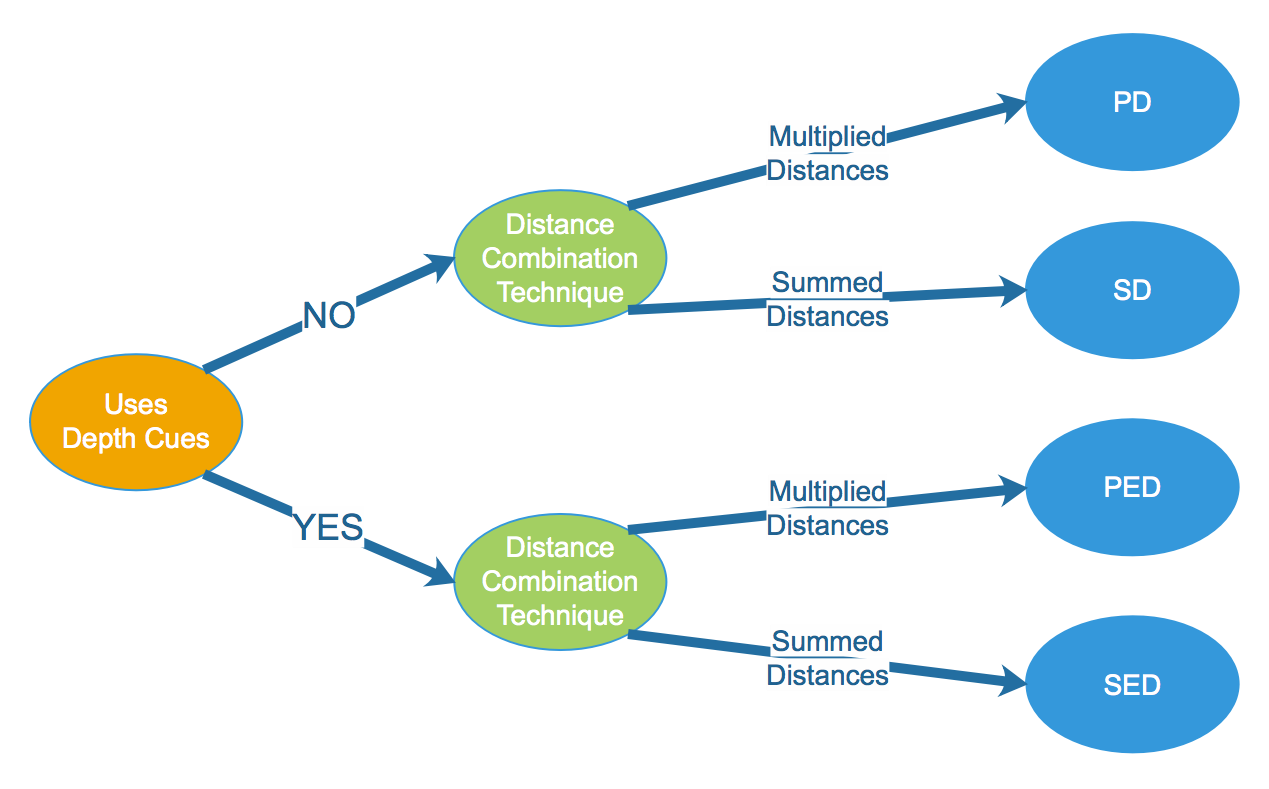
\includegraphics[width=0.7\linewidth] {implementation/affinities/modes}
   \label{fig:cars_w}
\end{center}
\caption[Affinity Pipeline Modes]{An visualization of all affinity computation modes that can be run by our pipeline. Abbreviations \textbf{PD} and \textbf{PED} stand for product of distances, whereas the additional \it{E} in PED stands for euclidean and hints that we are using Euclidian, metric units instead pixel units. Similarly, \textbf{SD} and \textbf{SED} stand for summed (euclidean) distances. Please note that affinity matrices generated by the mode SD or SED can only be used in combination with the \textit{Kernighan-Lin} segmentation method but affinities generated by running the modes PD and PED can be used together with spectral clustering and min-cut.}
\label{fig:affinity_modes}
\end{figure}
When running the mode \textbf{PD} or \textbf{PED} (the so called \textbf{P-affinity} modes) we combine distance by multiplying them. The affinity matrix is computed according to the definition of equation $\ref{eq:prod_dist_affinity}$. However, when running the mode \textbf{SD} or \textbf{SED} the distances are summed and the corresponding affinity is computed as defined in equation $\ref{eq:sum_dist}$. \\ \\
Additionally, our pipeline also offers a mode to compute affinities between shortly disconnected trajectories. The idea is to prepend (extend) one additional tracking point to a predecessor (successor) frame by adding the average motion distance of the next (previous) five frames to the trajectory's starting point (end point). Please note that this run-mode is only is optional and thus has to be invoked manually. Moreover, we could not observe any improvements in the resulting segmentations, when enabling this mode. \\ \\ 
In summary, the affinity matrix is computed between a trajectory and every other trajectory by calculating the distances described above and then combining them in a certain way. Every trajectory instance therefore carries a list of affinities, which are sorted by their partner trajectory's label in an ascending order. \\ \\
Therefore, for building the affinity matrix, we fetch all used trajectories, order them by their label value (again, ascending). Then, all we have to do is to traverse these ordered trajectories and then write their ordered affinities (to the other trajectories) into a file. Actually, each trajectory forms a line, where a line consists of the affinity values of the currently visited trajectory. Our writer uses a special file formatter that is able to generate a Matlab readable mat file. The pairwise affinities for $n$ valid trajectories result in an $n \times n$ affinity matrix $W$ as shown in figure $\ref{fig:cars_affinity_matrix}$. \\ \\
\begin{figure}[H]
\begin{center}
   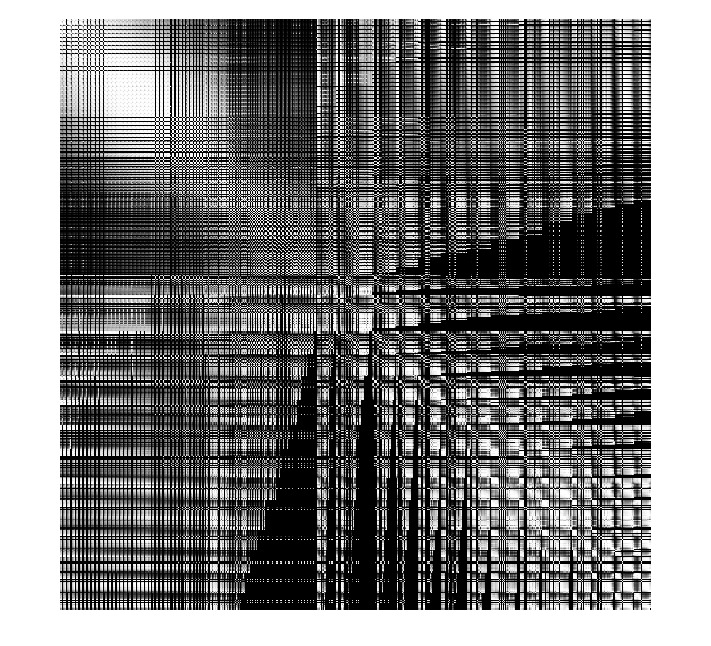
\includegraphics[width=0.65\linewidth] {implementation/affinities/cars/cars_w}
   \label{fig:cars_w}
\end{center}
\caption[Affinity Matrix]{Visualization of affinities among trajectories and the structure of the matrix $W$. The affinity is visualized by a grayscale image. The row-and column indices in the matrix determine a trajectory pair and the value at that position their affinity. Bright values indicate a high affinity between two trajectories.}
\label{fig:cars_affinity_matrix}
\end{figure}
To later support queries that allow to fetch affinities by a trajectory label, we also have to write a file containing every valid trajectory label identifiers. The labels are in an ascending order with respect to their label id. Figure $\ref{fig:affinity_index_label_mapping}$ shows how an affinity lookup by two given trajectory labels can be performed.
\begin{figure}[H]
\begin{center}
   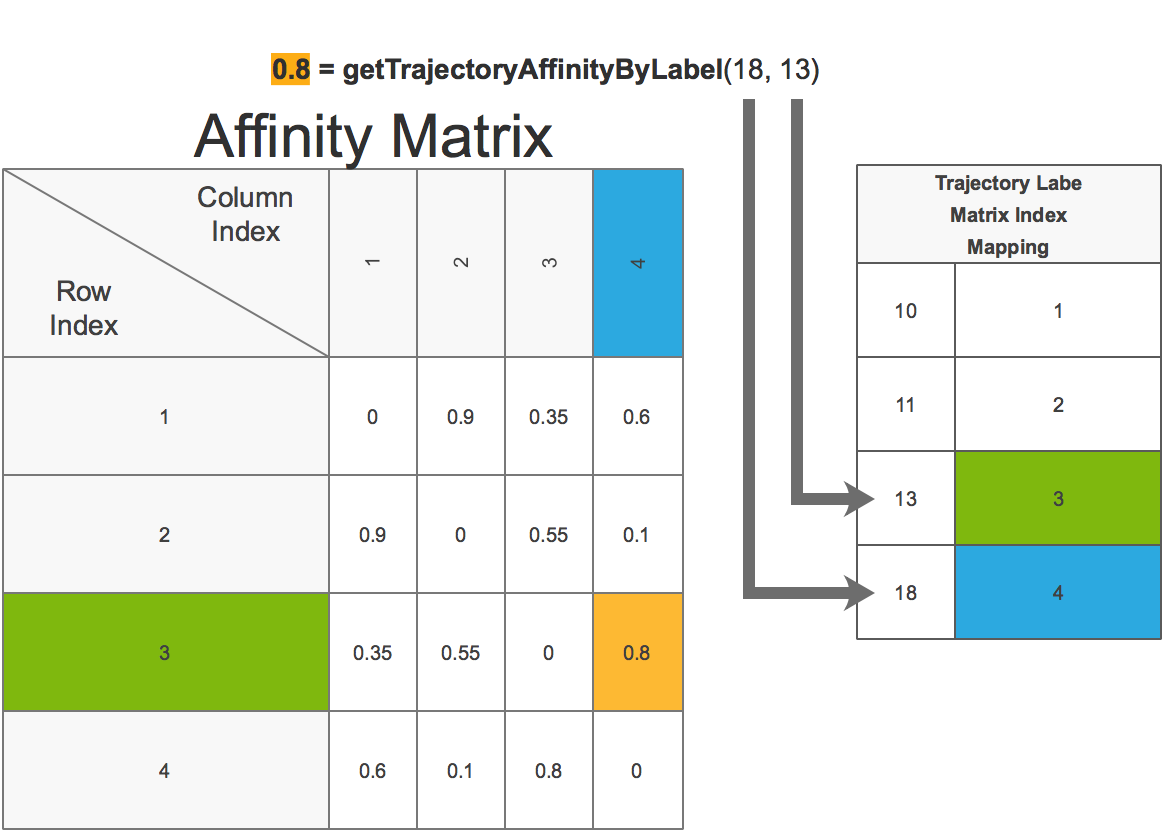
\includegraphics[width=0.85\linewidth] {implementation/affinities/affinity_label_mapping}
   \label{fig:cars_w}
\end{center}
\caption[Mapping between Affinity Matrix Indices and Trajectory Labels]{In order to lookup an affinity value between two trajectories we first have to lookup their matrix indices. This is performed loading a file that contains a mapping between the trajectory-labels and affinity matrix-indices. In this example, we want to get the affinities between the trajectories with the label id 18 and id 13. We first look those label's matrix indices and then use those indices to lookup the actual affinity value.}
\label{fig:affinity_index_label_mapping}
\end{figure}
Apart from generating the affinity matrix our pipeline also extracts the per trajectory nearest neighboring trajectories. The distance to those neighbors is measured with respect to the average spatial distance. Luckily, we already have computed this spatial distance value while traversing the trajectory pairs. \\ \\
To conclude this section and offer the reader a better understanding what those affinities actually are and mean, we discuss an affinity visualization, produced by our pipeline, shown in figure $\ref{fig:cars_affinities}$.
\begin{figure}[H]
\begin{center}
\subfigure[Similarities Car Foreground]{
   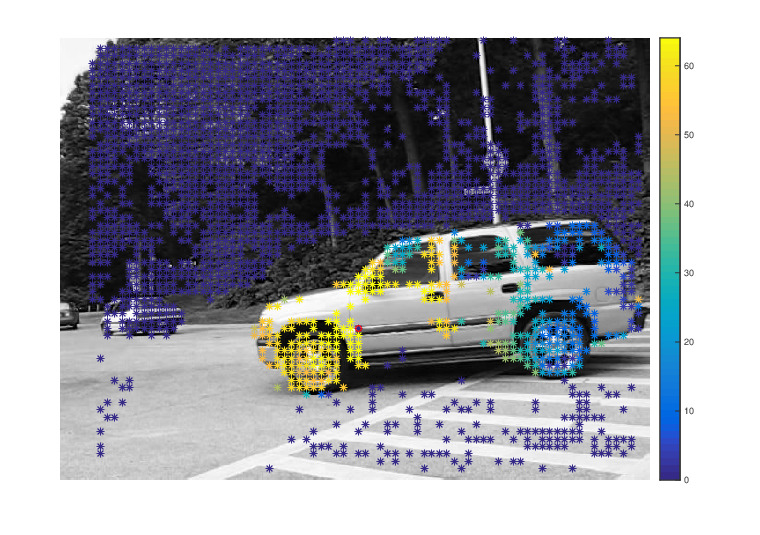
\includegraphics[width=0.48\linewidth] {implementation/affinities/cars/fc}
   \label{fig:cars_a}
}
\subfigure[Similarities Car Background]{
   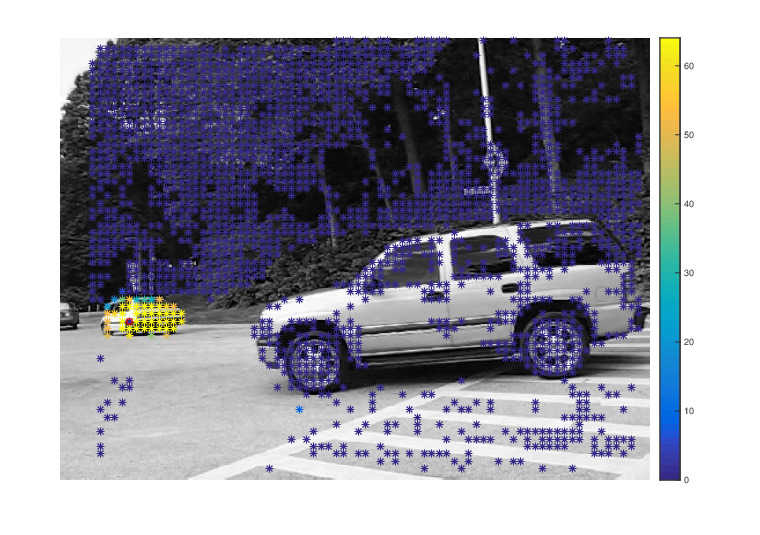
\includegraphics[width=0.48\linewidth] {implementation/affinities/cars/cb}
   \label{fig:cars_b}
}
~
\subfigure[Similarities Woods]{
   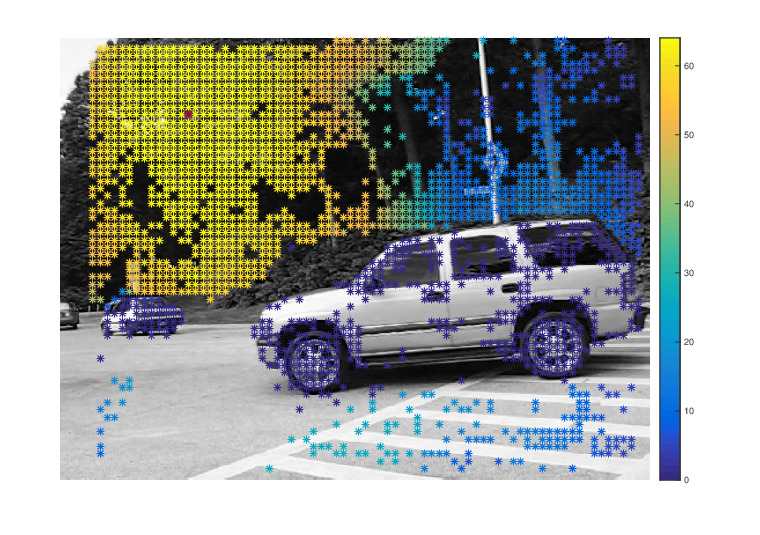
\includegraphics[width=0.48\linewidth] {implementation/affinities/cars/woods}
   \label{fig:cars_c}
}
\subfigure[Similarities Street]{
   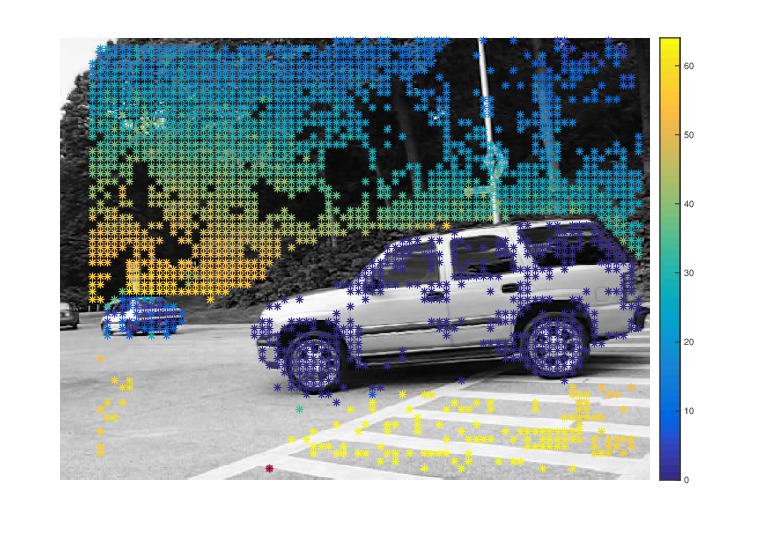
\includegraphics[width=0.48\linewidth] {implementation/affinities/cars/street}
   \label{fig:cars_d}
}
\end{center}
\caption[Trajectory Affinities Example]{Visualizing four examples of the affinities between a selected trajectory point (marked in red) and its affinities to any other present trajectory point. The more similar two points are, the more yellowish a dot get. Contrary, the more dissimilar two points are, the more bluish the point gets.}
\label{fig:cars_affinities}
\end{figure}
In this figure, we visualize four examples of the affinity values between a selected point (marked by a red dot) and every other trajectory. The larger the similarity, the more yellow the color becomes and, vice versa,  the smaller the affinity, the more blue is becomes. For example in subfigure $\ref{fig:cars_b}$, we selected a point on the moving car in the background. It has strong affinities to tracked points within the car and small to the front car and to the background. Similar results are shown in the other subfigures. This results hints the potential of our pipeline. \\ \\
In the next section we will discuss methods that use the previously generated output to generate a sparse motion segmentation.

\section{Sparse Motion Segmentation}
\label{sec:sparse_motion_segmentation}
In this section we explain how we generate sparse motion segmentations using the previously calculated affinity matrix. \\ \\
\begin{figure}[H]
\begin{center}
\subfigure{
   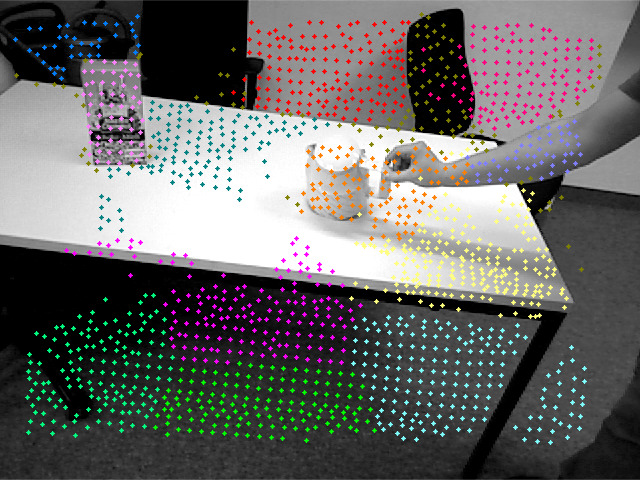
\includegraphics[width=0.31\linewidth] {implementation/segmentation/preword/bonn_cereal}
}
\subfigure{
   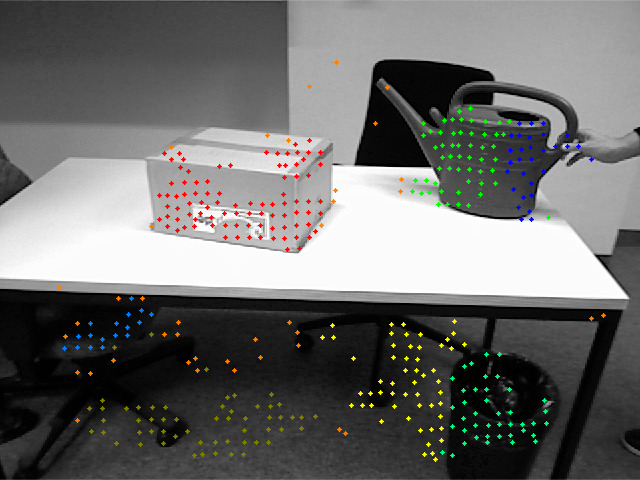
\includegraphics[width=0.31\linewidth] {implementation/segmentation/preword/bonn_watercan}
}
\subfigure{
   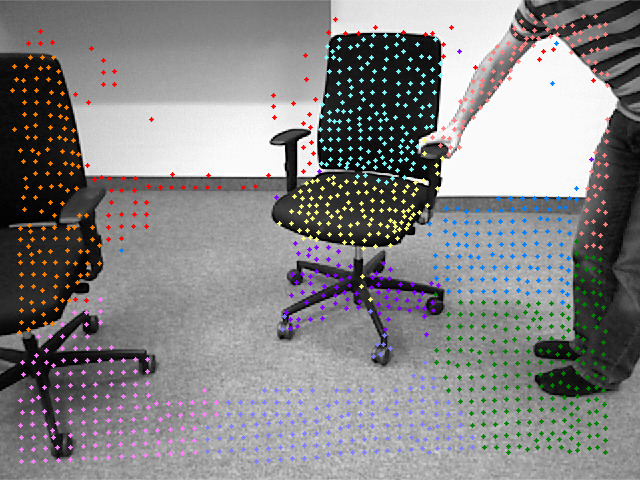
\includegraphics[width=0.31\linewidth] {implementation/segmentation/preword/bonn_chairs}
}
\end{center}
\caption[Sparse Segmentations]{Sparse motion segmentations produced by our pipeline.}
\label{fig:sparse_segmentations}
\end{figure}
In fact, our pipeline supports three different segmentation methods, all having their pros and contras. In particular can can perform the task of motion segmentation using spectral clustering of the affinity matrix (\textbf{SC}), building a graph of the affinity matrix and calculating several cuts via min-cut (\textbf{MC}) or lastly, by using the affinities to solve the graph partitioning problem using the Kernighan-Lin Heuristic (\textbf{KL}). \\ \\
Every implemented segmentation method returns a file containing a mapping between the trajectory label and their segment label. This allows to draw motion segmentations resulting by our segmentation methods. \\ \\
In order to draw the segmentation of the $k-th$ dataset frame, we load all trajectories that are active in that frame. For a trajectory, being active in a certain frame refers to a trajectory, which contains a point that was tracked in that particular frame. To draw the segmentation image of frame $k$, we iterate over each trajectory and select their tracking points that are currently active in frame $k$. For each such tracking point we use its tracking position as the \textit{draw to position} and the label of its parent trajectory defines the color that should be used to draw the pixel. Some resulting segmentations, produced by our pipeline, are shown in figure $\ref{fig:sparse_segmentations}$.\\ \\
In the following we offer a detailed explanation of these motion segmentation methods.
\subsection{Spectral Clustering}
In the previous section we described how the pairwise affinities can be computed. For $n$ trajectories we ended up by a a $n \times n$ affinity matrix $W$. \\ \\ 
One possible way to interpret these matrix entries is to identify them as edge weights of a fully connected graph $G$, where each trajectory represents a node. Following this interpretation, then, the task of extracting the moving objects  corresponds to the task of grouping several similar graph vertices. \\ \\
An approximately optimal partitioning of $G$ can be obtained via spectral clustering as described in section $\ref{sec:spectral_clustering_bg}$. The idea behind this approach is to decompose the Laplacian matrix $L$ that corresponds to $W$ into its eigenvalues and eigenvectors $V$ and then run k-means on $V$. We used algorithm $\ref{alg:spectral_clustering_algorithm}$ in Matlab to run such a spectral clustering. As the very first step we load the affinity matrix $W$ and compute its normalized Laplacian according to the definition from equation $\ref{eq:normalized_graph_laplacian}$. Next, we compute the eigen-decomposition of $L$, defined as
\begin{equation}
	V^{T} \Lambda V = L^{\text{sym}}
\end{equation}
by using Matlab's fast eigen-decomposition $\textit{eigs}$. To get a better idea of how such eigenvectors might look like, please have a look at figure $\ref{fig:eigenvectors_laplacian_matrix}$.
\begin{figure}[H]
\begin{center}
\subfigure[Eigenvector Front Car]{
   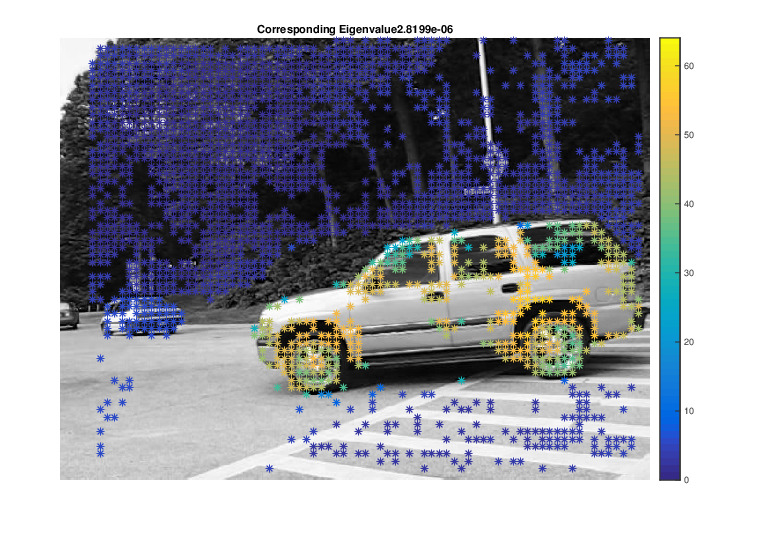
\includegraphics[width=0.48\linewidth] {derivation/eigenvectors/cars/ev_cf}
   \label{fig:cars_eigenvectors_laplacian_a}
}
\subfigure[Eigenvector Background Car]{
   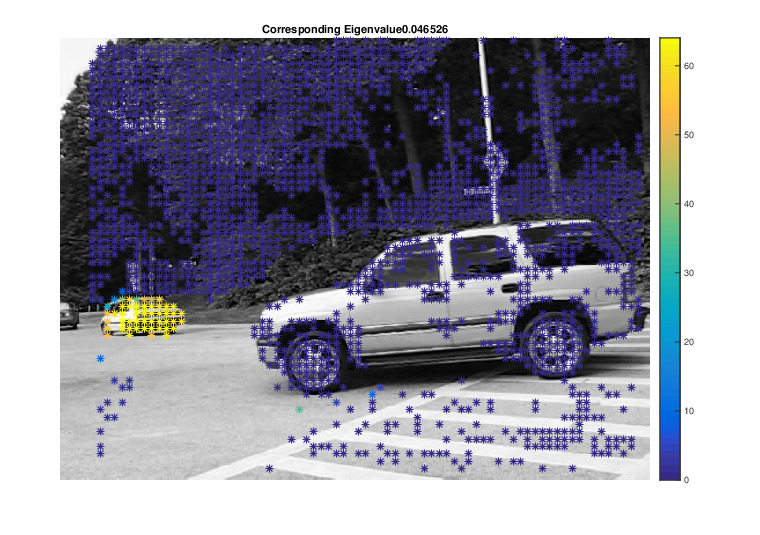
\includegraphics[width=0.48\linewidth] {derivation/eigenvectors/cars/ev_cb}
   \label{fig:cars_eigenvectors_laplacian_b}
}
\end{center}
\caption[Eigenvectors of Laplacian Matrix]{Visualizing the two smallest eigenvector of the Laplacian matrix computed on the cars dataset. Each component of an eigenvector maps to exactly one trajectory. More yellow values indicate a large value, whereas bluish markings indicate a low value. The actual value does not matter. However, we already observe local groupings of moving objects/their parts, when visualizing the eigenvectors.}
\label{fig:eigenvectors_laplacian_matrix}
\end{figure}
The actual clustering is performed on the eigenvectors of $L$. In fact, we further assume that we only need some of the eigenvectors for the clustering. Actually, it can be proven, that at least $k$ eigenvectors are required if there are $k$ segments$\footnote{In fact, the background is also counted as a segment. The actual proof shows, that to extract the k connected components in a graph, we need to run a spectral clustering on the k smallest eigenvectors.}$. Therefore, we select the $m$ smallest eigenvectors $V_m$ according to their $\lambda \in \Lambda$. \\ \\
The final clustering is performed by running k-means, similar as described in section $\ref{sec:k_means}$, on $V_m$ using a pre-specified number of clusters. To run k-means, we use a random initialization. Since we might end up at a local minima, we run the k-means algorithm 200 times and take the result with the smallest error$\footnote{The error is measured in terms of the distance between the resulting cluster centers and their assigned feature points.}$
The output of this method is a grouping of vector indices of the eigenvectors $V_m$. Each index that belong to the same group correspond to the same moving object. To obtain the corresponding trajectory label that maps to a certain vector index, we perform a query similar as shown figure $\ref{fig:affinity_index_label_mapping}$ by using the \textit{index-label-mapping} list. \\ \\ 
The actual choice for the number of $m$ and the clusters we want to solve for can be specified by the user. \\ \\
The limitation of this approach is that such a clustering is only defined for non-negative affinity values between trajectories. Otherwise the eigenvalue decomposition of the Laplacian would yield complex valued eigenvectors. In practise, this assumption means that it is easy to specify which trajectories should be in the same cluster but it is impossible to impose that they should be separated. Moreover, the described spectral clustering is supposed to produce oversegmentations and there is not always smooth a transitions between the eigenvectors produced, when clustering them.

\subsection{Minimum Cut} 
\label{sec:min_cut_seg}
In this section we describe an alternative method to generate motions segmentation. This approach directly addresses some issues of the previously described spectral clustering approach. \\ \\
Generally, eigenvectors typically show smooth transitions within a region and more or less clear edges between regions. Unfortunately, the k-means algorithm cannot properly deal with this setting. Its results generally suffer from oversegmentations since it approximates smooth transitions by multiple constant functions. Furthermore, the optimal number of clusters $K$ is by no means obvious, because clusters are represented by many eigenvectors. \\ \\
To address this issue, we formulate an energy, similar as in $\cite{Bro10c}$, that comprises a spatial regularity term. By minimizing this energy term we obtain the optimal segmentation assignment. \\ \\
Initially, we again load the affinity matrix $W$, but this time together with the extracted trajectory's nearest neighbors $\mathcal{N}$. The actual number of trajectory neighbors is a user-tuneable parameter. The fewer neighbors a trajectory gets assigned to, the faster the pipeline runs. However, keep in mind that the number of neighbors determines the segmentation quality. Usually, one third of the total trajectory count is a solid choice for the neighborhood size. \\ \\ 
Analogously, as we did in the spectral clustering section, we transform $W$ to the normalized Laplacian and decompose it into its eigenvalues and eigenvectors. Again, the number of eigenvectors and clusters we want to solve for have to be specified by the user. \\ \\
In the following we describe this energy term, but before doing so, we have to provide the reader some definitions. Let $v_i^a$ denote the $a$-th component of the $i$-th eigenvector and $\textbf{v}^a$ the vector compose of the $a$-th components of all m extracted eigenvalues. Notice that the index a maps to a distinct trajectory. Let $\mathcal{N} \left( a \right)$ denote the neighboring trajectories of trajectory a, which were initially loaded. For a fixed number of clusters $K$, we want to compute the optimal trajectory assignments $\pi^{a} \in \{ 1, \dots , K \}$ such that the energy formulated in equation $\ref{eq:min_cut_energy_revisited}$ is minimized.
\begin{equation}
\begin{aligned}
& E \left( \pi, K \right) = \underbrace{\sum_{A} \sum_{k=1}^K \delta_{\pi^A, k} \norm{\bf{v}^A - \mu_k}_{\lambda}}_\text{data term} + \underbrace{\nu \sum_A \sum_{B \in \mathcal{N}(A)} \frac{1- \delta_{\pi^A, \pi^B}}{\norm{\bf{v}^A - \bf{v}^B}}}_\text{smoothness term} \\
& \text{where } \norm{\bf{v}^A - \bf{\mu}}_\lambda = \sum \frac{v_i^A -  \mu_i}{\lambda_i}
\end{aligned} 
\label{eq:min_cut_energy_revisited}
\end{equation}
The $\delta_{\pi^A, \pi^B}$ is a characteristic function which is equals one if the trajectories $A$ and $B$ are assigned to the same cluster and zero otherwise. Similarly, the expression $\delta_{\pi^A, k}$ is a boolean function that is one, if the trajectory $A$ got the label k assigned. \\ \\
The $\textbf{data term}$ models an unary cost that is minimized by k-means, where $\mu_k$ denotes the centroid of cluster $k$. Notice that this term makes use of the norm $\norm{.}_{\lambda}$. In this norm each eigenvector is weighted by the inverse of the square root of its corresponding eigenvalue. Such a weighting ensures that eigenvectors that separate more distinct clusters correspond to smaller eigenvalues. \\ \\
The $\textbf{smoothness term}$ acts as a regularizer that penalizes the spatial boundaries between clusters. The penalty is weighted by the inverse difference of the eigenvectors along these boundaries. On one hand, this penalty is very small for the case when there are clear discontinuities along cluster boundaries. On the other hand, boundaries within a smooth area are penalized for more heavily. This avoids splitting clusters at arbitrary locations due to smooth transitions in the eigenvectors. \\ \\
The parameter $\nu$ acts as the tread-off between the two terms and thus determines how smooth the final segmentation should be. \\ \\
Minimizing the energy formulated energy in equation $\ref{eq:min_cut_energy_revisited}$ is a difficult problem, because it exhibit many local minima. However, when using a fixed number of clusters $K$, then minimizing this energy becomes a multi-label Markov Random Field (MRF) optimization problem with unknown centroids.
\begin{figure}[H]
\begin{center}
\subfigure[Initialization]{
   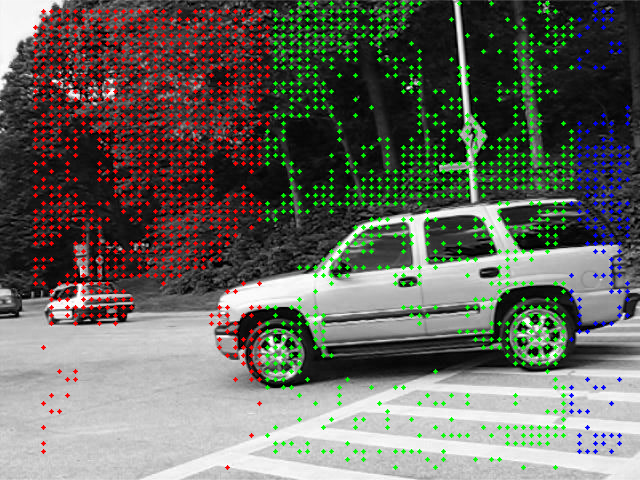
\includegraphics[width=0.15\linewidth] {implementation/mc/0}
   \label{fig:convergence_mc_seg_0}
}
\subfigure[Iteration 1]{
   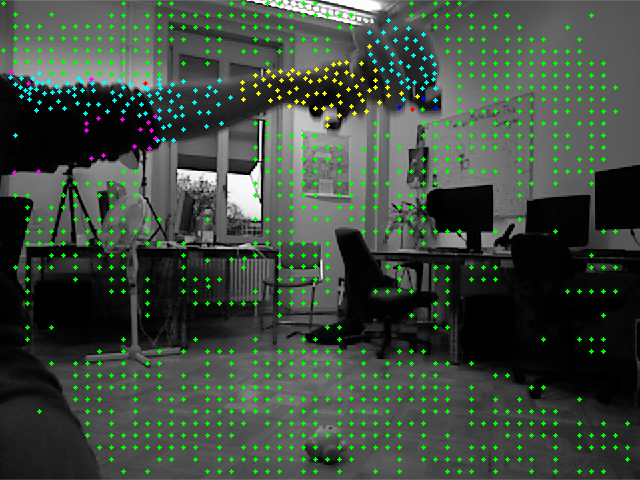
\includegraphics[width=0.15\linewidth] {implementation/mc/1}
   \label{fig:convergence_mc_seg_1}
}
\subfigure[Iteration 2]{
   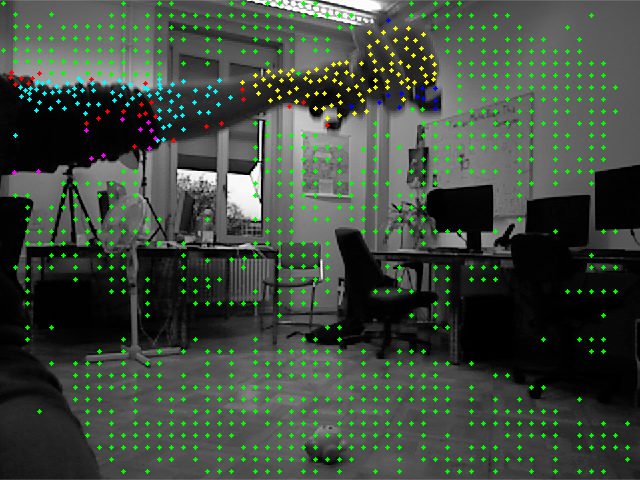
\includegraphics[width=0.15\linewidth] {implementation/mc/2}
   \label{fig:convergence_mc_seg_2}
}
\subfigure[Iteration 3]{
   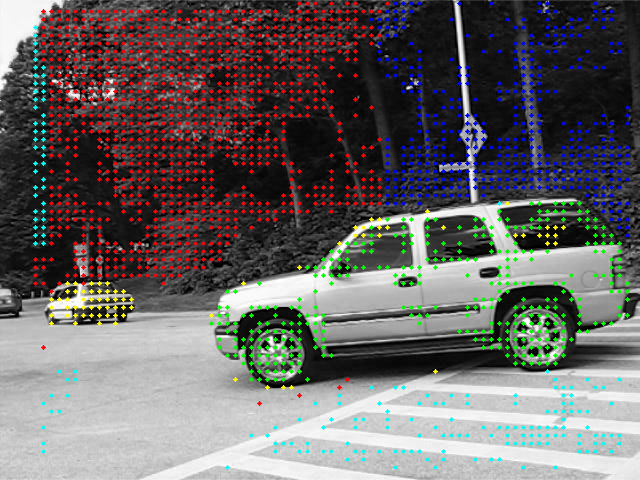
\includegraphics[width=0.15\linewidth] {implementation/mc/3}
   \label{fig:convergence_mc_seg_3}
}
\subfigure[Iteration 4]{
   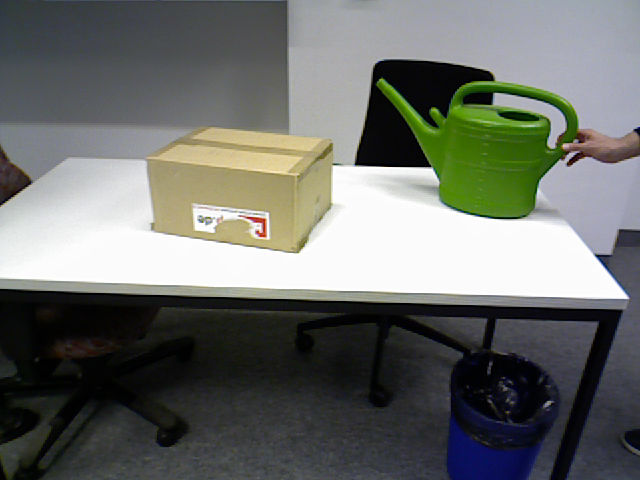
\includegraphics[width=0.15\linewidth] {implementation/mc/4}
   \label{fig:convergence_mc_seg_4}
}
\end{center}
\caption[Convergence MC]{Visualizing the convergence of MC applied on the cars dataset.}
\label{fig:convergence_mc_seg}
\end{figure}
In our Matlab implementation we optimize this minimization problem by using an iterative solver. But before starting this iteration, we initialize the cluster centroids with an equidistant labeling defined as
\begin{equation}
	\forall k \in \{ 1, \dots, K \} \forall A_i : (k - 1) \frac{n}{K} \leq i \leq k \frac{n}{K} : \pi^{A_i} = k
\label{eq:initialization_min_cut}
\end{equation}
An loop iteration consists of two main steps: In the first step, we fix the label assignments and solve for the cluster centroids by running k-means. In the second step, we fix the centroids by using the previously computed centers and optimize for the assignments by running a multi-label graph cut energy minimization. For this purpose we rely on $\cite{Fulkerson2009}$'s $\textit{GCMex}$ framework$\footnote{This frameworks offers some handy methods to compute the multi-label graph cut.}$, which is a freely available Matlab implementation. We repeat this iteration until the labels assignments have converged. The resulting assignment is the motion segmentation. An example of the MC segmentation method is shown in figure $\ref{fig:convergence_mc_seg}$. 

\subsection{Kernighan-Lin Heuristic} 
In this section we describe a method that addresses the problem of motion segmentation by formulating it as a minimum cost multi-cut problem on a trajectory similarity graph as defined in section $\ref{sec:similarity_graphs}$. The energy term we optimize to find an optimal graph partition is based on the work presented in $\cite{KB15b}$. To solve this graph cut problem numerically we implemented the $\textit{Kernighan-Lin}$ heuristic ($\textbf{KL}$) described in $\cite{Ker70}$. \\ \\
% WIP
In the following, let $G = (E, V)$ denote an undirected graph, where $V$ is the set of vertices and $E$ the set of edges. Moreover, every edges in $E$ has a certain weight $e_c$ assigned. Then, the minimum cost multi-cut problem decomposes the graph $G$ into an optimal number of segments such that the overall edge weights cost is minimized. Equivalently, this vertex labeling problem can be formulated as a binary edge labeling problem, which is defined as
\begin{equation}
\begin{aligned}
& \min_{y \in \{0,1 \}^{|E|}} \sum_{e \in E} c_e y_e \\
& \text{subject to } y \in \text{MC}
\end{aligned}
\end{equation}
The expression $\text{MC}$ denotes the set of characteristic functions of all multi-cuts and thus corresponds to all $y \in \{0,1 \}^{|E|}$ that form closed boundaries. Hence, such boundaries represent a valid decomposition of the graph. To define these characteristics a series of cycle inequalities, similar as done in $\cite{Chopra1993}$, are formulated as defined in the follows:
\begin{equation}
	\forall C \in \text{cycles}(G) \forall e \in C: y_e \leq \sum_{e^{'} \in C \backslash \{e\}} y_{e^{'}}
\end{equation}
Furthermore, in $\cite{Chopra1993}$ it was shown, that it is sufficient to only consider those cycles in which each vertex is only connected to its successor and predecessor. \\ \\
In order to avoid trivial solutions when optimizing for these characteristics, we employ the following edge weighting strategy: Typically, we chose the weights such that edges which should be cut are negative and positive for those which are connected to vertices that should be joined.
In the following, let us assume that we know the edge cut probabilities $p_e$. In that case the negative function
\begin{equation}
	\text{logit}\left( p_e \right) = \log \left( \frac{p_e}{1 - p_e} \right)
	\label{eq:logit_function}
\end{equation}
provides such a desired behavior. A plot if the negative logit function defined as in $\ref{eq:logit_function}$ is shown in figure $\ref{fig:negative_logit_function}$.
\begin{figure}[H]
\centering
\begin{tikzpicture}[trim axis left]
\begin{axis}[
  axis x line=center,
  axis y line=center,
  grid=both,
  xtick={-2,-1,...,1,2},
  ytick={-2,-1,...,1,2},
  xlabel={$x$},
  ylabel={$-\text{logit}\left( x \right)$},
  xlabel style={below right},
  ylabel style={above left},
  no markers,
  xmin=-0.5,
  xmax=1.5,
  ymin=-1.5,
  ymax=1.5]
\addplot +[thick, domain=0:1] {-log10(x/(1-x)};
\end{axis}
\end{tikzpicture}
\caption[Logit Function Plot]{A plot of the negative logit function applied on the domain [0,1].}
\label{fig:negative_logit_function}
\end{figure}
If $p_e < 0.5$ then $\text{logit}\left( p_e \right) > 0$ and thus the according edge cost $c_e$ is positive and therefore the edge $e$ is expensive to be cut out from the graph. Conversely, in case that $p_e > 0.5$ the negative logit function of $p_e$ is smaller than zero and thus it is beneficial to cut e. \\ \\
For computing pseudo-probabilities, we use the inverse of the logit function, the so called \textit{logistic function}
\begin{equation}
	f(z) = \frac{1}{1 + \exp \left( -z \right)}.
	\label{eq:logistic_function}
\end{equation}
This function can therefore be used to define pseudo cut probabilities. Next we have to determine what the input value $z$ represents. Clearly, $z$ is equals to the result of the logit function applied on the psuedo-probability. However, such a definition is not helpful at all, since we defined $f(z)$ as the inverse of the logit, thus end up with a recursive definition. Another interpretation of the negative logit is that is models distances between edges. If the distances are too large, a cut should be performed. A distance $d$ that can be used is the one resulting when computing S-affinities as stated in equation $\ref{eq:sum_dist}$. The final expression for $z$ is defined as:
\begin{equation}
	z = d - \log \left( \frac{p}{1-p} \right) + \log \left( \frac{\tilde{p}}{1-\tilde{p}} \right).
\label{eq:edge_dist_weights}
\end{equation}
where $p$ is a fixed cut probability and set equals $0.5$ and $\bar{p}$ is a parameter denoting the prior cut probability. If $\bar{p}$ is increased, more edges will be cut and the number of resulting segments increases. Choosing a small $\bar{p}$ results in an undersegmentation. \\ \\
In the following we use discussed formulation to model the similarity graph. In particular we compute its edge weights by using the definition from equation $\ref{eq:edge_dist_weights}$. Using such negative and positive weights allow to optimize for the correct number of moving objects including small objects that show discriminative motion in a small number of frames. This approach is supposed to produce more reliable results than the segmentation method described in the section spectral clustering.
\begin{figure}[H]
\begin{center}
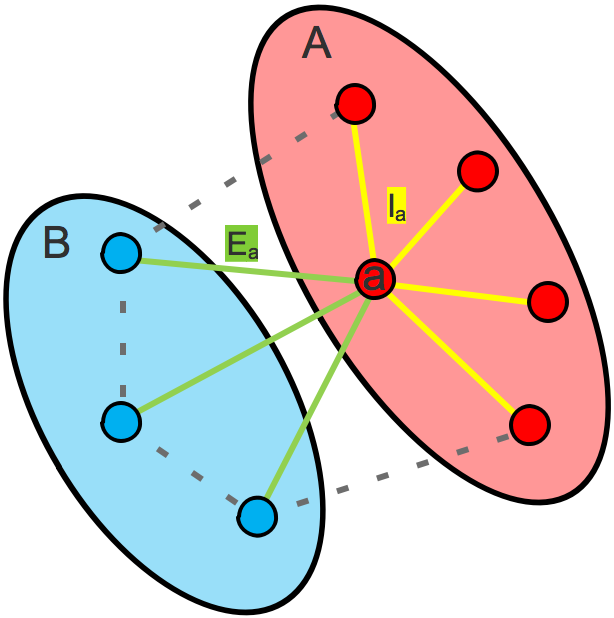
\includegraphics[width=0.6\linewidth] {implementation/segmentation/kl_energies}
\end{center}
\caption[KL Energy Terms]{Visualization of the internal $I_a$ and external costs $E_a$ of a vertex $a \in A$.}
\label{fig:kl_partition_energies}
\end{figure}
Next, let us discuss an algorithm that allows to partition the similarity graph discussed before. The Kernighan-Lin heuristic $KL$ is a good candidate for this task. This algorithm attempts to find a partition of $V$ into two disjoint subsets $A$ and $B$ of equal size, such that the sum $T$ of edge weights between the vertices in $A$ and $B$ is minimized similar as shown in figure $\ref{fig:kl_partition_energies}$. For defining the cost, let $I_a$ be the internal cost of the vertex $a \in A$, which is defined as the sum of the costs of the edges between $a$ and other nodes in $A$. Furthermore, let $E_a$ denote the external cost of $a$, which is defined as the sum of the costs of edges between $a$ and the vertices in $B$. The balance of a vertex is given by the difference defined in equation $\ref{eq:kl_d_values}$.
\begin{equation}
	D_a = E_a - I_a
\label{eq:kl_d_values}
\end{equation}
If $a$ and $b$ are interchanged, then the reduction in cost is equals.
\begin{equation}
	T_{n} - T_{n-1} = D_a + D_b - 2c_{a,b}
\label{eq:kl_difference_ext_int_costs}
\end{equation}
Note that $c_{a,b}$ in equation $\ref{eq:kl_difference_ext_int_costs}$ defines the cost of the possible edge between $a$ and $b$. \\ \\
The $KL$ algorithms attempts to find an optimal series of interchange operations between the elements in $A$ and $B$, which maximizes the value of equation $\ref{eq:kl_difference_ext_int_costs}$. The determined optimal operation sequence is then executed to compute the partition of the graph into the sets $A$ and $B$. \\ \\
In the following we offer reader some details about the \emph{Kernighan-Lin} heuristic formulated in algorithm $\ref{alg:kernighan_lin}$. 
\begin{algorithm}[H]
\caption{Kernighan-Lin}
\begin{table}[H]
  \begin{tabular}{@{}lll@{}}
    \textbf{Input:} & Graph \emph{G = (V, E)} \\
    \textbf{Output:} & Binary Graph Partition $\left( A, B \right)$ \\
  \end{tabular} 
\end{table}
\setlength{\fboxrule}{0pt} 
\begin{boxedminipage}{1.0\textwidth}
  \begin{algorithmic}[1]
  	  \State $\text{Determine initial balanced vertex partition into sets A, B}$
      \Do
		\State $\forall a \in A, \forall b \in B: \text{Compute D values}$
		\State $\text{Let gv, av, bv be empty lists}$
		\For{$\text{n=1 to } |V|/2$}
			\State $\text{Find } a \in A, b \in B \text{ such that } g = D_a + D_b - 2e_{a,b} \text{ is maximal}$
			\State $\text{Remove a and b from further consideration in this pass}$
			\State $\text{Put g to gv, a to av, b to bv}$
			\State $\text{Update D values for all elements of } A = A \backslash \{a\}, B = B \backslash \{b\}$
		\EndFor
		\State $\text{Find k that maximizes } g_{max} = \sum_{i=1}^k gv_i$
		\If{$g_{max} > 0$} 
			\State $\text{Exchange } av_1,\dots, av_k \text{ with } bv_1,\dots, bv_k$  
		\EndIf	
      \doWhile{$g_{max} > 0$}
  \end{algorithmic}
  \end{boxedminipage}
  \vskip1.5pt
\label{alg:kernighan_lin}
\end{algorithm}
In this algorithm, we initialize two vertex sets according to some rule. In the inner loop, we determine a ranking of the vertices according to their gain. First, we compute equation $\ref{eq:kl_d_values}$ on every vertex. Then, we compute the gain between all vertices $a \in A$ and $b \in B$ according to the formulation in equation $\ref{eq:kl_difference_ext_int_costs}$ and select the vertices $a$ and $b$ that produces the largest gain value. Please notice that this can yield negative values. Next, we remember their gain value, mark them as dirty and put each of these vertices into special sets $av$ and $bv$. Afterwards the D values of every all vertices that are not dirty are updated. We have to repeat this procedure $|V|/2$ times since the each set $A$ and $B$ contains that many vertices. \\ \\
In the list of gains we look for the maximal partial sum of gains. The index in the gain list that produced the maximum sum is used as the permutation index for performing a series of interchange operation. Working with this partial sums makes sense, since, as long as the sum increases, the gain in the next iteration got bigger. Permuting till the max partial sum would result in having a lower gain in the next outer iteration. We repeat the steps of the most outer loop until there is no more gain. \\ \\
Our Java implementation initially loads the corresponding $\textit{S-affinity}$ matrix and its corresponding nearest neighbor list. Then, an internal undirected graph $G = \left( V, E \right)$ is constructed. Its vertices represent thereby individual trajectories and two vertices are connected if their are actual neighbors. The edge weights are the actual affinity values between two vertices. Usually, the full neighborhood the is loaded into the pipeline and thus the complete graph is formed, i.e. every vertex is interconnected with any other vertex. However, the number of neighbors per trajectory, that should be loaded into the pipeline, can be directly specified by a user via a neighborhood size parameter. \\ \\ 
So far, our KL method is only capable to perform a binary partition on a graph. However, we would like to extend it in a way, such that it can partition a graph into an arbitrary number of labels. \\ \\
To address this problem we apply a greedy strategy. Let us assume we want to solve for $k$ clusters and we are working with $n$ vertices. Then, we distribute the n vertices according to some initialzation rule among k empty sets. Then, for each possible pair of subsets we sequentially run algorithm $\ref{alg:kernighan_lin}$ giving us the pairwise optima. We repeat this procedure until the solution has converged. Our final $KL$ algorithm we use to solve the multi-cut problem is listed in algorithm $\ref{alg:kl_multiple_segments}$.
\begin{algorithm}[H]
\caption{Kernighan-Lin Multicut Heuristic}
\begin{table}[H]
  \begin{tabular}{@{}lll@{}}
    \textbf{Input:} & Graph \emph{G = (V, E)} \\
        & Number of segments C \\
    & Number of repetitions N  \\
    & Number of dummy vertices D \\
	\textbf{Output:} & Multiple Graph Partition $\left( A_1,\dots, A_N \right)$ 
  \end{tabular} 
\end{table}
\textbf{Procedures:} $KernighanLin(G)$  \\
\setlength{\fboxrule}{0pt} 
\begin{boxedminipage}{1.0\textwidth}
  \begin{algorithmic}[1]
  	\For{$n = 1 : N$}
  	  \State $\text{Split V into C initial balanced sets} A_1,\dots,A_C$
  	  \State $\text{Append D dummy vertices to each initial set} A_k$ 
      \ForAll{$\text{distinct vertex set pair} \left( A_k, A_l\right)$}
        \State $ \text{Form the subgraph } G_{k,l} = (V, E)$
		\State $\text{Run } KernighanLin(G_{k,l}) \text{ and Update G}$
      \EndFor
    \EndFor{$\text{d}$}
  \end{algorithmic}
  \end{boxedminipage}
  \vskip1.5pt
\label{alg:kl_multiple_segments}
\end{algorithm}
In our implementation we want to use the following initialization: One set among the k sets is initialized with all n vertices and the other sets are empty. This will give every set the same change to get some vertices in a fair amount of time. However, this also violates our restriction that \textit{the subsets have to be of equal size}. The solution to this problem is to introduce so called dummy vertices, which are basically placeholders and exhibit zero similarities. Meaning, that they do not affect the cost terms used during the optimization.

\section{Dense Motion Segmentation}
\label{sec:dense_motion_segmentation}
Up to this moment we are able to generate sparse motion segmentations by using three different methods. However, in some vision related tasks, it would actually make sense to determine dense masks. This would enable us to extract the moving objects by simply applying the corresponding mask. However, keep in mind that generating dense motion segmentations is not the focus of this work. Therefore, we also will not evaluate this method. \\ \\
In this section we describe a simple method to produce a dense motion segmentations from previously generated sparse segmentations. \\ \\
For this purpose we adapted an existing implementation, which address the problem of demosaicing an image by formulating it as convex optimization problem. The problem is reformulated in its primal-dual form and an iterative solver was developed. I developed this program during a semester project in the class \textit{Convex Optimization} in 2015 held by Prof. Dr. P. Favaro at the unversity of Bern. The class is based in the book convex optimization $\cite{BoydVanderberg2004}$. \\ \\
A detailed derivation can be found in the appendix $\ref{chap:appendix_demosaicing}$. The class, as well as the implementation and the derivation assume a certain background in convex problem formulations and how to solve such problems. \\ \\
The idea is to interpret the sparse segmentation as in image a image with missing data due to its sparsity. Therefore, we want to solve the problem of hole filling, which is the same as finding the demosaiced image, using our formulation. \\ \\
For a given image with missing data $g$ we want to find its reconstructed image $u$. This can be achieved by minimizing an energy term $E$ which is defined as 
\begin{equation}
	E(u) = \underbrace{\norm{\nabla u}_2}_{\text{smoothness term}} + \frac{\lambda}{2} \underbrace{\norm{u - g}^2_{\Omega}}_{\text{data term}}	
\end{equation}
where we defined the data term as
\begin{equation}
\begin{aligned}
& \norm{u - g}^2_{\Omega_{C}} = \sum_x \sum_y \Omega_{C}(x,y)\norm{u(x,y) - g(x,y)}^2 \\
& \text{where } \Omega_{C}(x,y)= 
\begin{cases}
    0,& \text{if } $g(x,y)$ \text{ is missing}\\
    1,              & \text{otherwise}
\end{cases}
\end{aligned}
\end{equation}
First let us have a look at the \textbf{data term}. It ensures that the reconstructed image does not deviate too much from the given input $g$ w.r.t the norm $\norm{\cdot}_\Omega$. The reason for introducing this kind of norm is that we want to define a meaningful measure that captures the sense of meaningful. Therefore, we have to skip every invalid image location in $g$, when applying this norm on the difference between $u$ and $g$. The \textbf{smoothness term} ensures a smooth transition between the colors in the image.
\begin{figure}[H]
\begin{center}
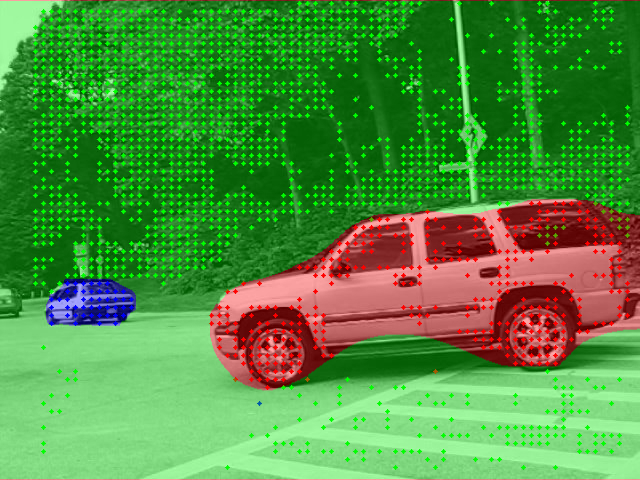
\includegraphics[width=0.8\linewidth] {implementation/dense_seg/cars_1}
\end{center}
\caption[Dense Segmentation Cars]{A dense segmentation produced by our pipeline. We see an overlay of the sparse segmentation on top of the dense masks. As we can see, the dense segmentation is basically a blur of the initial given sparse segments.}
\label{fig:dense_segmentation_cars_1}
\end{figure}
In section $\ref{sec:primal_dual_form}$ describe how to solve this optimization problem by formulating its primal-dual form. Such a formulation allows us to derive an iterative solver to address this optimization. A detailed, step by step derivation can be found in the appendix $\ref{chap:appendix_demosaicing}$. One iteration of our solver runs the following steps:
\begin{equation}
\begin{aligned}
	y^{n+1} &= \frac{y^n + \sigma \nabla \bar{x}^{n}}{\max{\left(1,\twonorm{y^n + \sigma \nabla \bar{x}^{n}} \right)}} \nonumber \\
	x^{n+1} &= \frac{x^n - \tau \left[ \left( \partial_x y_{x}^{n+1} + \partial_y y_{x}^{n+1} \right) + \left( \partial_x y_{y}^{n+1} + \partial_y y_{y}^{n+1} \right) \right] +  \tau \lambda \Omega g}{1+\tau \lambda \Omega} \\
	\bar{x}^{n+1} &= x^{n+1} + \theta(x^{n+1} - x^n)
\end{aligned}
\end{equation}
For computing $\nabla$ we use a forward difference approximation scheme.
We repeat this update rule until $\norm{\bar{x}^{n+1} - \bar{x}^{n}}$ is small enough. Moreover, we use the parameter assignment listed in equation $\ref{eq:parameter_set_up}$. \\ \\
An dense segmentation produced by running this method is shown in figure $\ref{fig:dense_segmentation_cars_1}$. This figure shows the dense segments as colored masks. Additionally, we also show the sparse segmentation, using the same colors. As we can see, the dense segmentation is basically a blurred version of the initial sparse input. 